\documentclass{article}
\usepackage{amsmath}
\usepackage{amsthm}
\usepackage{amssymb}
\usepackage{pgfplots}
\usepackage{amsfonts}
\usepackage[margin=2.5cm]{geometry}
\usepackage{graphicx}
\usepackage[export]{adjustbox}
\usepackage{fancyhdr}
\usepackage[portuguese]{babel}
\usepackage{hyperref}
\usepackage{lastpage}

\pagestyle{fancy}
\fancyhf{}

\hypersetup{
    colorlinks,
    citecolor=black,
    filecolor=black,
    linkcolor=black,
    urlcolor=black
}

\newtheorem*{sol*}{\underline{Solu\c c\~ao:}}
\newtheorem*{proof*}{\underline{Prova:}}
\renewcommand\qedsymbol{$\blacksquare$}

\rfoot{P\'agina \thepage \hspace{1pt} de \pageref{LastPage}}

\title{EXERC\'ICIOS DE C\'ALCULO}
\author{Renan Wenzel}
\date{\today}

\begin{document}

\begin{figure}[ht]
	\minipage{0.76\textwidth}
		
\includegraphics[width=4cm]{icmc.png}
		\hspace{5cm}
		
\includegraphics[height=4.9cm,width=4cm]{brasao_usp_cor.jpg}
	\endminipage	
\end{figure}

\begin{center}
	\vspace{1cm}
	\LARGE
	UNIVERSIDADE DE S\~AO PAULO

	\vspace{1.3cm}
	\LARGE
	INSTITUTO DE CI\^ENCIAS MATEM\'ATICAS E COMPUTACIONAIS - ICMC

	\vspace{1.7cm}
	\Large
	\textbf{EXERC\'ICIOS DE C\'ALCULO}

	\vspace{1.3cm}
	\large
	\textbf{Renan Wenzel - 11169472}

	\vspace{1.3cm}
	\large
	\textbf{Tha\'is Jord\~ao - tjordao@icmc.usp.br}

	\vspace{1.3cm}
	\today
\end{center}

\newpage

\tableofcontents

\section{N\'umeros Reais, Fun\c c\~oes e Introdu\c c\~ao a Limites}
\subsection{Exerc\'icios de Fun\c c\~oes e Panorama Geral}
\subsubsection{Exerc\'icio 1}  
\paragraph{}Parte 1 - Se considerarmos 
$$
f(x) = \frac{x^3 + x^2 - x - 1}{x-1}, x\neq{1},
$$
ent\~ao a que classe de fun\c c\~oes ela pertence? Note que se efetuarmos a divis\~ao polinomial, concluiremos que 
$$
\frac{x^3 + x^2 - x - 1}{x-1} = x^2 + 2x + 1.
$$
Isto significa que f \'e uma fun\c c\~ao polinomial de grau 2? Justifique e fa\c ca o passo-a-passo.
\begin{proof*}
	Considere a fun\c c\~ao 
	$$
	f(x) = \frac{x^3 + x^2 - x - 1}{x-1}, x\neq{1},
	$$
	e $p(x) = x^3 + x^2 - x - 1, q(x) = x - 1,$ em que $p:\mathbb{R}\rightarrow\mathbb{R}$ e $q(x)\mathbb{R}/\{1\}\rightarrow\mathbb{R}$ s\~ao polin\^omios. Segue que:
	$$
	f(x) = \frac{x^3 + x^2 - x - 1}{x-1} = \frac{p(x)}{q(x)}, x\neq{1}.
	$$
	Por defini\c c\~ao, uma fun\c c\~ao na forma de quociente de polin\^omios, em que o denominador \'e um polin\^omio com o dom\'inio tal que ele nunca \'e nulo, \'e conhecida como uma fun\c c\~ao racional. 

	No entanto, \'e melhor lidar com fra\c c\~oes de polin\^omios simplificados, ou seja, \'e preciso encontrar o fator comum entre ambos. Observe que, em x = 1, 
	$$
	p(x) = 1^3 + 1^2 - 1 - 1 = 1 + 1 - 1 - 1 = 0
	$$ 
	e 
	$$
	q(x) = 1 - 1 = 0,
	$$ 
	ent\~ao (x-1) \'e um fator comum entre ambos, isto \'e, ele pode ser fatorado ap\'os manipular o polin\^omio p(x) . Assim, note que, somando e subtraindo fatores para que possamos fatorar (x-1) de p(x), chegamos em: 
	$$
	p(x) = x^3 + x^2 - x - 1 = x^3 + (2x^2 - x^2) +(x - 2x) -1 = (x-1)(x^2 + 2x^2 + 1) = q(x)(x^2 + 2x^2 + 1),
	$$
	de forma que:
	$$
	f(x) = \frac{x^3 + x^2 - x - 1}{x-1} = \frac{p(x)}{q(x)} = \frac{q(x)(x^2 + 2x^2 + 1)}{q(x)} = x^2 + 2x^2 + 1, x\neq{1}.
	$$
	Logo, ap\'os efetivada a divis\~ao, obtemos que f \'e uma fun\c c\~ao polinomial de grau 2. 
\qedsymbol
\end{proof*}

\newpage

\paragraph{}Parte 2 - Verifique as seguintes identidades:
\begin{figure}[h!]
	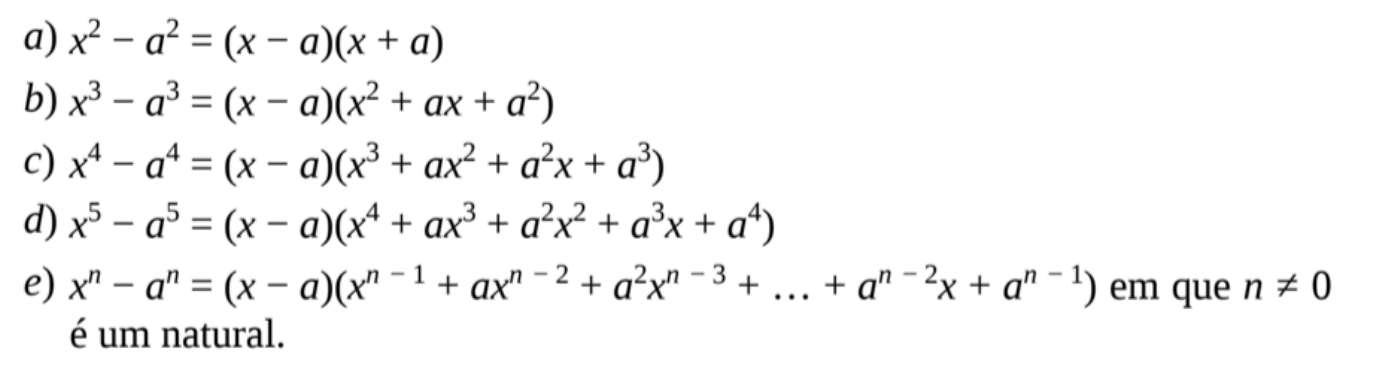
\includegraphics[width=15cm, height=4cm]{identidades.png}
\end{figure}

\begin{proof*}
	Antes da formaliza\c c\~ao da prova, um bom come\c co \'e analisar a imagem cuidadosamente. De fato, ao fazer isso, observe a repeti\c c\~ao do termo (x - a) \`a direita de cada igualdade. Outro ponto not\'avel \'e que, para cada n, ocorre uma expans\~ao de $\sum_{i=0}^{n}a^ix^{n-i-1}$ ao lado de (x - a), em que $n\in\mathbb{N}$. Em outras palavras, isso est\'a indicando fortemente a presen\c ca de uma hip\'otese indutiva para demonstrar o resultado. 
	
	Com  efeito, provemos o caso base do item a, ou seja, n = 2. Considere o produto (x-a)(x+a):
	$$
	(x - a)(x + a) = x^2 + xa - ax - a^2 = x^2 + ax - ax - a^2 = x^2 - a ^2.
	$$
	Destarte, obtivemos o caso base como verdadeiro. Nessa linha de racioc\'inio, a hip\'otese indutiva afirma que, dado uma base verdadeira, o resultado ser\'a provado se, assumindo o caso n-1 como verdade, o caso n tamb\'em ser\'a (pois assim, o caso 1 sendo verdadeiro implica que o 2 tamb\'em \'e, consequentemente o 3, o 4, etc.). Suponha que o resultado vale para n - 1, isto \'e, para $n\neq{0}$ 
	$$	
	x^{n - 1} - a^{n - 1} = (x - a)\biggl(\sum_{i=0}^{n-2}a^ix^{n-i-2}\biggr).
	$$
	Em part\'icular, somando $2a^{n-1}, $segue que:
	$$
	x^{n - 1} + a^{n - 1} = (x - a)\biggl(\sum_{i=0}^{n-2}a^ix^{n-i-2}\biggr) + 2a^{n-1}.
	$$
	Multiplicando ambos os lados por (x-a), chegamos em:
	$$
	(x - a)\biggl(\sum_{i=0}^{n-1}a^ix^{n-i-1}\biggr)  = (x - a)(x^{n-1} + \biggl(\sum_{i=1}^{n-2}a^ix^{n-i-1}\biggr) + a^{n-1})  = (x - a)(x^{n-1} + a^{n-1} + \biggl(\sum_{i=1}^{n-2}a^ix^{n-i-1}\biggr))  = 
	$$
	$$
	= (x - a)(2a^{n-1} + (x - a)\biggl(\sum_{i=0}^{n-2}a^ix^{n-i-2}\biggr) + \biggl(\sum_{i=1}^{n-2}a^ix^{n-i-1}\biggr))  = (x - a)(2a^{n-1} + x^{n-1} - a^{n-1} + \biggl(\sum_{i=1}^{n-2}a^ix^{n-i-1}\biggr)) = 
	$$
	$$
	= 2xa^{n-1} - 2a^n + (x-a)\biggl(x^{n-1} - a^{n-1} + \biggl(\sum_{i=1}^{n-2}a^ix^{n-i-1}\biggr)\biggr) = 2xa^{n-1} - 2a^n + x^{n} - xa^{n-1} -a^{n-1}x + a^{n} + (x-a)\biggl(\sum_{i=1}^{n-2}a^ix^{n-i-1}\biggr)\biggr) = 
	$$
	$$
	= xa^{n-1} - a^n + x^{n} - xa^{n-1} + (x-a)\sum_{i=1}^{n-2}a^ix^{n-i-1} = (x^n - a^n) + (xa^{n-1} - ax^{n-1} + (x-a)\sum_{i=1}^{n-2}a^ix^{n-i-1}) .
	$$
Analisemos o termo $(x-a)\sum_{i=1}^{n-2}a^ix^{n-i-1}$ antes de prosseguir. Temos:
	$$
	(x-a)\sum_{i=1}^{n-2}a^ix^{n-i-1} = x\sum_{i=1}^{n-2}a^ix^{n-i-1} - a\sum_{i=1}^{n-2}a^ix^{n-i-1} = \sum_{i=1}^{n-2}a^ix^{n-i} - \sum_{i=1}^{n-2}a^{i+1}x^{n-i-1} = 
	$$
	$$
	= ax^{n-1} + a^2x^{n-2} + \cdots + a^{n-2}x^2 - a^2x^{n-2} - ... -a^{n-2}x^2 - a^{n-1}x = ax^{n-1} - a^{n-1}x.
	$$
Juntando isso com a conta anterior, chegamos, finalmente, em:
	$$
	(x^n - a^n) + (xa^{n-1} - ax^{n-1} + (x-a)\sum_{i=1}^{n-2}a^ix^{n-i-1}) = (x^n - a^n) + (xa^{n-1} - ax^{n-1} + ax^{n-1} - a^{n-1}x ) =
	$$
	$$
	= x^n - a^n + 0 = x^n - a^n.
	$$
Portanto, 
	$$
	(x - a)\biggl(\sum_{i=0}^{n-1}a^ix^{n-i-1}\biggr) = x^n - a^n.
	$$
Agora que provamos isso, utilizando n = 3, 4, 5, mostramos as identidades que faltam:
\begin{itemize}
\item[n=3:] $$ x^3 - a^3 = (x-a)\sum_{i=0}^{2}a^ix^{2-i} = (x-a)(a^2 + ax + x^2). $$
\item[n=4:] $$ x^4 - a^4 = (x-a)\sum_{i=0}^{3}a^ix^{3-i} = (x-a)(a^3 + a^2x + ax^2 + x^3). $$
\item[n=5:] $$ x^5 - a^5 = (x-a)\sum_{i=0}^{4}a^ix^{4-i} = (x-a)(a^4 + a^3x + a^2x^2 + ax^3 + x^4).$$
\end{itemize}
\qedsymbol	
\end{proof*}

\subsubsection{Exerc\'icio 2} 
\paragraph{}Parte 1 - Fazendo todos os detalhes e explicando todos os passos, explicite o dom\'inio de cada umas das fun\c c\~oes abaixo e calcule os produtos $f\cdot{}g, g\cdot{}h \text{ e } h\cdot{}i$, em que:
$$
f(x) = 2x^3 - 5x^2 + 3, \hspace{0.5cm}
g(x) = 3x^2 - x + 2, \hspace{0.5cm}
h(x) = \frac{x^2 - 1}{x - 3} \hspace{0.2cm} \text{\&} \hspace{0.2cm}   
i(x) = \frac{x^3 - 1}{x^2 + 1}
$$
\begin{sol*}
A priori, analisemos os dom\'inios de cada uma das fun\c c\~oes. Come\c cando por f, levando em conta que, quando n\~ao explicitado, o dom\'inio de uma fun\c c\~ao \'e o maior subconjunto de $\mathbb{R}$ em que faz sentido defin\'i-la, temos $D_f = \mathbb{R}$, pois a fun\c c\~ao n\~ao possui pontos problem\'aticos (com isso, queremos dizer um ponto em que, por exemplo, ter\'iamos $\frac{1}{0}$ ou $\sqrt{-x}, x > 0$ e $x\in\mathbb{R}.$) Analogamente, segue que o dom\'inio de g tamb\'em \'e $D_g = \mathbb{R}.$ 

Contudo, ao lidarmos com os dom\'inios de h e i, \'e necess\'ario ter cautela, j\'a que s\~ao definidas por fra\c c\~oes. No caso de h, seu dom\'inio \'e o conjunto dos reais tais que x - 3 n\~ao \'e nulo, ou seja, 
$$
D_h = \{x\in\mathbb{R}: x - 3 \neq 0\} = \mathbb{R}/\{3\}.
$$
Em primeira vista, o caso da fun\c c\~ao i pode parecer o mesmo, ou seja, que vai ser definido como o conjunto dos reais a menos de um conjunto finito de pontos. No entanto, note que, para isso, seria preciso que $x^2 + 1 = 0, x\in\mathbb{R},$ o que nunca acontece (nos reais!). Portanto, i est\'a definido em $D_{i} = \mathbb{R}$.

Ademais, a forma de realizar produtos entre fun\c c\~oes deve ser esclarecida: O produto entre duas fun\c c\~oes f e g, definido ponto-a-ponto, \'e dado por
$$
(f\cdot{g})(x) = f(x) \cdot{g(x)}.
$$
Com isso em mente, vamos aos c\'alculos:
\begin{itemize}
\item[i.)] $f\cdot{g}$ (produto de f com g)
$$
(f \cdot{g})(x) = f(x)\cdot{g(x)} = (2x^3 - 5x^2 + 3)\cdot(3x^2 - x + 2) = 2x^3(3x^2 - x + 2) - 5x^2 (3x^2 - x + 2) + 3(3x^2 - x + 2) = 
$$
$$
= 6x^5 - 2x^4 + 4x^3 - 15x^4 + 5x^3 - 10x^2 + 9x^2 - 3x + 6 = 6x^5 - 17x^4 + 9x^3 - x^2 + 6
$$
\item[ii.)]$g\cdot{h}$  (produto de g com h)
$$
(g\cdot{h})(x) = g(x)\cdot{h(x)} = (3x^2 - x + 2)\cdot\biggl(\frac{x^2 - 1}{x - 3}\biggr) = \biggl(\frac{(3x^2 - x + 2)(x^2 - 1)}{x - 3}\biggr) = 
$$
$$
= \biggl(\frac{3x^4 - 3x^2 - x^3 + x + 2x^2 - 2}{x - 3}\biggr) = \biggl(\frac{3x^4 - x^2 - x^3 + x - 2}{x - 3}\biggr)
$$
\item[iii.)]$h\cdot{i}$ (produto de h com i)
$$
(h\cdot{i})(x) = h(x)\cdot{i(x)} = \biggl(\frac{x^2 - 1}{x - 3}\biggr)\biggl(\frac{x^3 - 1}{x^2 + 1}\biggr) = \biggl(\frac{(x^2 - 1)(x^3 - 1)}{(x - 3)(x^2 + 1)}\biggr) 
$$
$$
= \biggl(\frac{x^5 - x^2 -x^3 + 1}{x^3 + x - 3x^2 - 3}\biggr) 
$$
\end{itemize}
\qedsymbol
\end{sol*}

\paragraph{}Parte 2 - Sabendo que $\sin{x}$ n\~ao \'e uma fun\c c\~ao racional, mostre que a fun\c c\~ao $\tan{x}$ n\~ao pode ser uma fun\c c\~ao racional.
\begin{proof*}
A priori, sabemos que, para uma fun\c c\~ao ser racional, ela deve ser o quociente de dois polin\^omios. Analogamente, se uma fun\c c\~ao n\~ao \'e racional, ela n\~ao pode ser escrita como o quociente de dois polin\^omios. 

A posteriori, suponha que $\sin{x}$ n\~ao \'e uma fun\c c\~ao racional. Defina 
$$
\tan(x) = \frac{\sin(x)}{\cos(x)}.
$$
Desta forma, segue de cara que $\tan(x)$ n\~ao \'e uma fun\c c\~ao racional, pois um de seus componentes, no caso, $\sin(x)$, n\~ao pode ser escrito como o quociente de dois polin\^omios, de forma que, mesmo se $\cos(x)$ fosse racional, ainda assim seria imposs\'ivel escrev\^e-la como o quociente desejado. Portanto, a tangente $\tan(x)$ n\~ao pode ser uma fun\c c\~ao racional.
\qedsymbol
\end{proof*}

\subsubsection{Exerc\'icio 3}
\paragraph{}Parte 1  - Defina os conceitos de injetividade e sobrejetividade.
\begin{sol*}
Antes de defin\'i-los explicitamente, \'e importante conhecer um pouco de suas utilidades. O primeiro deles, a injetividade, lida com a quest\~ao da unicidade na imagem da fun\c c\~ao, tanto \'e que tamb\'em \'e conhecido como fun\c c\~ao 1-1, enquanto a sobrejetividade lida com o ``alcance'' da fun\c c\~ao. Se ambos os casos ocorrem, chamamos a fun\c c\~ao de bije\c c\~ao, uma classe muito importante pois ela relaciona cada elemento de cada um dos conjuntos (o dom\'inio e o contra-dom\'inio) unicamente, de forma que h\'a um inverso pra fun\c c\~ao, mas isso \'e outro t\'opico. 

Destarte, definamos ambas matematicamente. Dados dois conjuntos A e B n\~ao-vazios, seja $f:A\rightarrow{B}$ uma fun\c c\~ao entre os dois conjuntos. Dizemos que:
\begin{itemize}
\item[a)] f \'e uma fun\c c\~ao injetora se, para $a_1, a_2\in{A}, f(a_1) = f(a_2)$ implica que $a_1 =  a_2.$
\item[b)] f \'e uma fun\c c\~ao sobrejetora se, dado $b\in{B}$, existe (pelo menos) um elemento $a\in{A}$ tal que $f(a) = b.$
\end{itemize}

Com essas defini\c c\~oes em mente, retomemos o primeiro par\'agrafo. A unicidade mencionada segue pois, para uma aplica\c c\~ao qualquer de A em B ser uma fun\c c\~ao, ela precisa que, dados $a_1, a_2\in{A}$, caso $a_1 = a_2, f(a_1) = f(a_2)$. A injetividade diz o oposto, ou seja, se $f(a_1) = f(a_2), a_1 = a_2$. Juntando os dois, uma fun\c c~ao injetora obedece $f(a_1) = f(a_2) \text{ se, e somente se, } a_1 = a_2,$ dados $a_1, a_2\in{A},$ tal que cada elemento de um conjunto define unicamente um elemento no outro. Quanto \`a sobrejetividade, ela define quando uma fun\c c\~ao tem alcance m\'aximo, pois como cada $b\in{B}$ pode ser escrito como a fun\c c\~ao aplicada a algum elemento de A, segue que $B \subset f(A)$, tal que, como por defini\c c\~ao $f(A) \subset B$, temos $f(A) = B$, ou seja, a imagem da fun\c c\~ao \'e o contra-dom\'inio inteiro.
\qedsymbol
\end{sol*}

\paragraph{}Parte 2 - Mostre que a fun\c c\~ao $f(x) = \sin(x), x\in[0, \pi]$ n\~ao \'e injetora, mas para $x\in[0, \frac{\pi}{2}]$ ela \'e.
\begin{proof*}
Vamos mostrar uma contradi\c c\~ao engra\c cada. Suponha que, de fato, $f(x) = \sin(x)$ \'e injetora no intervalo $[0, \pi]$. Em particular, temos:
$$
\sin(0) = 0 = \sin(\pi) \Rightarrow 0 = \pi.
$$
Se isso fosse verdade, alguns desastres aconteceriam. Dentre eles, n\~ao existiriam c\'irculos, pois todos eles poderiam ser vistos como pontos, j\'a que sua \'area, $\pi\cdot{r^2} = 0$ para todo r, ou seja, tamb\'em n\~ao existiria engenharia e, quem sabe, nem mesmo o universo. Isso est\'a obviamente errado. Logo, $\sin(x)$ n\~ao pode ser injetora em $[0, \pi].$ 

De lado com os cataclismas e fins do mundo, considere, agora, o intervalo $[0, \frac{\pi}{2}].$ Sabemos que a fun\c c\~ao seno \'e estritamente crescente nesse intervalo, que \'e o primeiro quadrante. Assim, temos, para $x, y\in[0, \frac{\pi}{2}],$
$$
\sin(x) < \sin(y), x < y \text{ ou } \sin(x) > \sin(y), x > y.
$$
Assim, a \'unica forma de $\sin(x) = \sin(y)$ \'e quando x = y, que \'e a exata defini\c c\~ao de uma fun\c c\~ao injetora.
\qedsymbol
\end{proof*}

\paragraph{}Parte 3 - Fa\c ca as seguintes composi\c c\~oes: $f\circ{g}, g\circ{f}, f\circ{h} \text{ e } h\circ{f}$, em que:
$$
f(x) = -3x + 2, \hspace{0.5cm} g(x) = 3x^2 - x  + 2, \hspace{0.2cm} \text{ e } \hspace{0.2cm} h(x) = \frac{x^2 - 1}{x - 3}.
$$
\begin{sol*}
Antes de dar in\'icio \`as contas propriamente ditas, note que, ao compor h com f, ou f com h, o dom\'inio de f mudar\'a de $D_f = \mathbb{R}$ para $D_f = \mathbb{R}/\{3\}.$ Feita essa observa\c c\~ao, sigamos em frente:
\begin{itemize}
\item[i)]$$(f\circ{g})(x) = f(g(x)) = f(3x^2 - x + 2) = -3(3x^2 - x + 2) + 2 = -9x^2 + 3x - 6 + 2 = -9x^2 + 3x - 4.$$
\item[ii)]$(g\circ{f})(x)$
$$
(g\circ{f})(x) = g(f(x)) = g(-3x + 2) = 3(-3x + 2)^2 +3x - 2 + 2 =
$$
$$
= 3(9x^2 - 12x + 4) + 3x = 27x^2 - 36x + 12 + 3x = 27x^2 - 33x + 12.
$$
\item[iii)]$(f\circ{h})(x)$
$$
(f\circ{h})(x) = f(h(x)) = f(\frac{x^2 - 1}{x - 3}) = -3\biggl(\frac{x^2 - 1}{x - 3}\biggr) + 2 = 
$$
$$
= \frac{-3x^2 + 3}{x-3} + 2 = \frac{-3x^2 + 3 + 2x - 6}{x-3} = \frac{-3x^2 + 2x -3}{x-3}.
$$
\item[iv)]$(h\circ{f})(x) $
$$
(h\circ{f})(x) = h(f(x)) = h(-3x + 2) = \frac{(-3x + 2)^2 - 1}{-3x+2 - 3} = \frac{9x^2 -12x + 4 - 1}{-3x -1} = -\frac{3(3x^2 - 4x + 1)}{3x+1}
$$
\end{itemize} 
\qedsymbol
\end{sol*}
\subsection{Um Panorama Geral}
\subsubsection{Exerc\'icio 4}
\paragraph{} Parte 1 - Quais s\~ao os dois principais problemas a que se refere o C\'alculo diferencial e integral?
\begin{sol*}
O c\'alculo pode ser visto como o estudo de ``infinitos'', ent\~ao, partindo desse princ\'ipio, \'e poss\'ivel iluminar a mente com rela\c c\~ao \`a resposta para essa pergunta. Nessa linha de racioc\'inio, o c\'alculo diferencial \'e apresentado, normalmente, com o problema de motiva\c c\~ao da reta tangente e do passo de uma fun\c c\~ao. Explicitamente falando, a busca do ponto \'unico para cada reta tangente e o que acontece com a fra\c c\~ao $\frac{\Delta{f(x)}}{\Delta{x}}$ quando $\Delta{x}$ fica cada vez menor, ou seja, como uma mudan\c ca at\'e a vizinhan\c c\a imediata de x afeta sua fun\c c\~ao f(x). Em ess\^encia, ambos os problemas s\~ao os mesmos, pois lidam com a taxa de varia\c c\~ao de x em n\'iveis infinitesimais, da\'i que vem a parte do c\'alculo diferencial que estuda infinitos, mas s\~ao as coisas infinitamente pequenas.

Tratando-se do c\'alculo integral, diferente da busca pela taxa de varia\c c\~ao, ele lida com as \'areas de gr\'aficos de fun\c c\~oes, isto \'e, como calcular a \'area de um gr\'afico arbitr\'ario. Para isso, a no\c c\~ao de infinito como mencionada previamenta aparece em forma de aproxima\c c\~oes cada vez mais finas por meio de ret\^angulos que possuem tamanhos maiores ou menores para uma dada sec\c c\~ao do gr\'afico. Quanto mais ret\^angulos forem usados, ou seja, quando menor forem seus tamanhos, mas maiores forem seus n\'umeros, melhor ser\'a a aproxima\c c\~ao da \'area de dada fun\c c\~ao, tal que, quando alcan\c cados infinitos ret\^angulos, a \'area da figura formada pelo gr\'afico \'e exata. Essa forma\c c\~ao de ret\^angulos cada vez menores tamb\'em pode ser compreendida como uma divis\~ao do intervalo da reta que representa o dom\'inio da fun\c c\~ao em partes iguais cada vez menores, tal que quanto maior o n\'umero de partes, melhor a aproxima\c c\~ao, at\'e que, novamente, com infinitas partes, chega-se no valor exato da \'area da fun\c c\~ao.
\qedsymbol
\end{sol*}

\paragraph{} Parte 2 - Utilize a constru\c c\~ao da secante ao gr\'afico para obter a tangente, em que $f(x) = x^5$, explicitando a reta tangente no ponto (a, f(a)) e deixando claro como obteve o coeficiente angular desta reta.
\begin{sol*}
Antes de tudo, lembre-se que uma reta secante a um gr\'afico \'e tal que ela passa por exatos dois pontos dele. Considerando que o que liga dois pontos \'e uma reta, a secante pode ser interpretada como a taxa de varia\c c\~ao da fun\c c\~ao em dois pontos $x, x_0\in{D_f}$ dados. Em outras palavras, se S for a secante, temos
$$
S = \frac{f(x) - f(x_0)}{x - x_0} = \frac{\Delta{f(x)}}{\Delta{x}}.
$$
Retome, agora, o exer\c c\'icio 4.1. A palavra "taxa de varia\c c\~ao" tamb\'em aparece l\'a, ent\~ao, consequentemente, a secante apareceu. Vamos seguir nessa linha de racioc\'inio, junto com a no\c c\~ao de infinitesimalidade, para obter a taxa de varia\c c\~ao imediata (Nome chique para derivada) de f no ponto $x_0$. Com efeito, a varia\c c\~ao imediata \'e o valor de S quando $x$ se torna $a$ e, para isso, utilizemos a no\c c\~ao de limite:
$$
\lim_{x\to{a}} S = \lim_{x\to{a}}\biggl(\frac{f(x) - f(a)}{x - a}\biggr) = \lim_{x\to{a}}\biggl(\frac{x^5 - a^5}{x - a}\biggr) = \lim_{x\to{a}}\biggl(\sum_{n=0}^{4}a^nx^{4-n}\biggr) = \sum_{n=0}^{4}a^n\lim_{x\to{a}}x^{4-n}= 
$$
$$
= \sum_{n=0}^{4}a^na^{4-n} = \sum_{n=0}^{4}a^{n+4-n} = \sum_{n=0}^{4}a^4 = 5a^4 .
$$
Como esse valor \'e exato e, consequentemente uma reta passando em um ponto s\'o, ele representa a tangente em (a, f(a)) com coeficiente angular igual a 5, pois a soma possui 5 termos, independentes do \'indice, $a^4$ iguais (apesar de n = 4, a soma come\c ca do 0, ent\~ao s\~ao n+1 = 5 termos). Esse processo pode, de fato, ser generalizado para um mon\^omio de grau n, $f(x) = x^n$, para obtermos que a tangente ao ponto $(x_0, f(x_0))$ \'e dada por $nx^{n-1}.$ Essa regra de obten\c c\~ao da tangente de um mon\^omio \'e mais conhecida como regra do tombo em cursos iniciantes, e \'e uma das bases para fazer a maioria das deriva\c c\~oes do C\'alculo diferencial. Uma observa\c c\~ao interessante, para finalizar, \'e o uso do exerc\'icio 1.1 parte 2 para chegar no resultado que quer\'iamos, sendo este o caso em que n = 4 dividido por (x - a).
\qedsymbol
\end{sol*}

\paragraph{} Parte 3 - Calcule a \'area de $f(x) = x^3$ dividindo o intervalo $[0, 1]$ em 7 parte iguais. Qual o valor aproximado da \'area a que se chega? Dividindo-se o intervalo em mais partes, digamos $\lfloor{\pi}\rfloor\cdot{10^{36}}$, espera-se que esta aproxima\c c\~ao do valor real da \'area melhore ou piore?
\begin{sol*}
A priori, dividiremos o intervalo em 7 partes iguais, ou seja, I = [0, 1] se quebra nos seguintes peda\c cos:
$$
I_1 = \biggl[0, \frac{1}{7}\biggr],     I_2 = \biggl[\frac{1}{7}, \frac{2}{7}\biggr],       I_3 = \biggl[\frac{2}{7}, \frac{3}{7}\biggr],    I_4 = \biggl[\frac{3}{7}, \frac{4}{7}\biggr],    I_5 = \biggl[\frac{4}{7}, \frac{5}{7}\biggr], I_6 = \biggl[\frac{5}{7}, \frac{6}{7}\biggr], I_7 = \biggl[\frac{6}{7}, 1\biggr].
$$
Agora, vejamos como a fun\c c\~ao f(x) se comporta neles, ou melhor, como sua \'area \'e influenciada por deslocamentos ao longo de cada peda\c co de I. O princ\'ipio por tr\'as desse processo \'e aproximar \'area por ret\^angulos menores que a total e depois por ret\^angulos maiores que ela. Comecemos, ent\~ao, por esses menores, ou seja, analisemos o valor de f nos pontos da esquerda dos intervalos. Em seguida, somaremos eles, dividindo pelo n\'umero de divis\~oes, no caso, 7, e repetiremos para os pontos \`a direita dos intervalos. Segue que 
$$
L_7 = \frac{1}{7}\biggl(f(0) + f(\frac{1}{7}) + f(\frac{2}{7}) + f(\frac{3}{7}) + f(\frac{4}{7}) + f(\frac{5}{7}) + f(\frac{6}{7})\biggr) =
$$
$$
\frac{1}{7}(0 + \frac{1}{7^3}(1^3 + 2^3 + 3^3 + 4^3 + 5^3 + 6^3)) = \frac{1}{7^4}\biggl(1^3 + 2^3 + 3^3 + 4^3 + 5^3 + 6^3\biggr) = \frac{441}{7^4}
= 0.183.$$
Repetindo o processo para os n\'umeros das pontas direitas dos intervalos, temos:
$$
R_7 = \frac{1}{7}\biggl(f(\frac{1}{7}) + f(\frac{2}{7}) + f(\frac{3}{7}) + f(\frac{4}{7}) + f(\frac{5}{7}) + f(\frac{6}{7}) + f(1)\biggr) =
$$
$$
\frac{1}{7}(\frac{1}{7^3}(1^3 + 2^3 + 3^3 + 4^3 + 5^3 + 6^3) + 1) = \frac{1}{7^4}\biggl(1^3 + 2^3 + 3^3 + 4^3 + 5^3 + 6^3\biggr) + \frac{1}{7} = \frac{441}{7^4} + \frac{1}{7}= 0.183 + 0.142 = 0.325.
$$
Assim, obtemos que a \'area da fun\c c\~ao, A, \'e tal que:
$$
L_7 < A < R_7.
$$
	\par{}Ademais, dividindo-se o intervalo em $3\cdot{10^{36}} = \lfloor{\pi}\rfloor\cdot{10^{36}}$ partes iguais, note que os ret\^angulos se tornam mais numerosos e com bases menores. Assim, a \'area individual de cada um deles ser\'a menor, tal que, ao som\'a-los, chegaremos em uma \'area mais aproximada, uma aproxima\c c\~ao mais refinada do valor da \'area da fun\c c\~ao. Isso esconde o principal mecanismo da soma de Riemann, ou seja, da defini\c c\~ao da Integral Definida, no sentido que, ao tomar a soma de Riemann, busca-se dividir os intervalos em um quantidade infinitamente pequena, tal que "ao chegar em infinito", a \'area, antes aproximada, torna-se exata. Este exemplo ilustra isso atrav\'es da compara\c c\~ao de intervalos antes n\~ao t\~ao pequenos (7 divis\~oes) com intervalos min\'usculos ($\lfloor{\pi}\rfloor\cdot{10}^{36}$ divis\~oes),
\qedsymbol
\end{sol*}


\section{Propriedades dos Limites, Limites Laterais, Limites de Determinadas Fun\c c\~oes, Fun\c c\~oes Cont\'inuas e Suas Propriedades}
\subsection{Continuidade e Limite}
\subsubsection{Exerc\'icio 1}
\paragraph{} Parte 1 - Classifique como verdadeira ou falsa a seguinte afirma\c c\~ao e demonstre ou d\^e um contra-exemplo.
``Se $f: \mathbb{R}\rightarrow\mathbb{R}$ \'e uma fun\c c\~ao, ent\~ao
$$
\lim_{x\to{1}}f(x) = f(1).\text{''}
$$
\begin{sol*}
Considere a seguinte fun\c c\~ao:
$$
f(x) = \left\{
\begin{array}{ll}
	x, &\quad \text{se } x\neq{1}\\
	9, & \quad \text{se } x=1.
\end{array}
\right.
$$

Seja $\epsilon > 0$ qualquer e analisemos a seguinte inequa\c c\~ao para $|x|\neq 1$:
$$
	|f(x) - 1| = |x - 1|.
$$
Com isso, tome $\delta = \epsilon$ e suponha que $0 < |x - 1| < \delta$, tal que x nunca ser\'a igual a 1. Com isso, segue que 
$$
	|f(x) - 1| = |x - 1| < \delta = \epsilon \Rightarrow |f(x) - 1| < \epsilon.
$$
Logo, $\lim_{x\to{1}}f(x) = 1$, mas f(1) = 9, mostrando que a afirma\c c\~ao \'e falsa.
\qedsymbol
\end{sol*}
\paragraph{} Parte 2 - \'E poss\'ivel, dada uma fun\c c\~ao $f:\mathbb{R}-\{\pi\}\rightarrow \mathbb{R}$, n\~ao definida no ponto $x=\pi$, calcular 
$$
\lim_{x\to\pi}f(x)?
$$
D\^e um exemplo e justifique.
\begin{sol*}
Ao definir um limite no ponto p, utilizamos o fato de p ser, por hip\'otese, ponto de acumula\c c\~ao do dom\'inio da fun\c c\~ao. Consequentemente, p n\~ao necessariamente precisa estar nesse dom\'inio para que possamos calcular o limite de f nele. Esse \'e o caso mais geral do que foi pedido no exerc\'icio, ent\~ao, para exemplificar, tome $f:\mathbb{R}-\{\pi\}\rightarrow\mathbb{R}$ como:
$$
f(x) = \left\{\begin{array}{ll}
	\sin(x) & \quad \text{se } x < \pi \\
	\sin(-x) & \quad \text{se } \pi < x
\end{array}\right.
$$
Note que a fun\c c\~ao est\'a definida em $\mathbb{R}-\{\pi\}.$ Com isso, seja $\epsilon > 0$ qualquer. Vamos calcular o limite por meio dos limites laterais, mostrando que eles s\~ao iguais quando x tende a $\pi$. Come\c cando pelo limite lateral \`a esquerda, note que
$$
|f(x) - 0| = |\sin(x) - 0| = |\sin(x) - 0| = |\sin(x)|< \epsilon.
$$
O $\epsilon$ ali pode ser visto como um meio para encontrarmos o $\delta$, j\'a que \'e o que precisamos fazer. Deixando isso de lado, manipularemos o m\'odulo como segue:
$$
|\sin(x)| < \epsilon \Rightarrow -\epsilon < \sin(x) < \epsilon \Rightarrow \sin^{-1}(-\epsilon) < x < \sin^{-1}(\epsilon).
$$
Subtraindo $\pi$ dos dois lados, obtemos
$$
\sin^{-1}(-\epsilon) - \pi < x - \pi < \sin^{-1}(\epsilon) - \pi.
$$
Foquemos no lado \`a esquerda primeiro, tal que, definindo $\delta_1 = \sin^{-1}(\epsilon) + \pi$, vale que, quando $-\delta_1 < x - \pi < 0$, 
$$
-\delta_1 = -\sin^{-1}(\epsilon) - \pi = \sin^{-1}(-\epsilon) - \pi < x - \pi.
$$
Pelo racioc\'inio acima, isso implica que 
$$
|f(x) - 0| < \epsilon,
$$
ou seja, 
$$
\lim_{x\to\pi^{-}}f(x) = 0.
$$
Por outro lado, quanto ao limite lateral \`a direita (isto \'e, $x > \pi$), observando a desigualdade obtida para o mesmo lado e definindo $\delta_2 = \sin^{-1}(\epsilon) - \pi $, se $0 < x - \pi < \delta_2$, temos:
$$
x - \pi < \delta_2 = \sin^{-1}(\epsilon) - \pi,
$$
donde segue que $|f(x) - 0| = |\sin(-x)| = |\sin(x)| < \epsilon$. Logo,
$$
\lim_{x\to\pi^{+}}f(x) = 0.
$$
Portanto, como os dois limites s\~ao iguais, segue que $\lim_{x\to\pi} f(x) = 0$, o que ilustre que \'e poss\'ivel calcular o limite em um ponto fora do dom\'inio da fun\c c\~ao.
\qedsymbol
\end{sol*}
\paragraph{} Parte 3 - Escreva formalmente o que significa uma fun\c c\~ao ser con\'tinua em um ponto de seu dom\'inio.
\begin{sol*}
	A ideia por tr\'as da continuidade \'e a falta de quebras no gr\'afico da fun\c c\~ao (em termo popular: pode ser desenhada sem tirar o l\'apis do papel). A deifni\c c\~ao matem\'atica por tr\'as dele procura preservar essa no\c c\~ao atrav\'es da ideia de que, n\~ao importa qu\~ao pr\'oximos sejam dois pontos, sempre \'e poss\'ivel fazer o gr\'afico da fun\c c\~ao neles igualmente pr\'oximos, ou seja, dados dois pontos da fun\c c\~ao, o erro da aproxima\c c\~ao tende a zero quando calcula-se ela nesses dois pontos. 

Rigorosamente falando, essas ideias s\~ao formuladas no jarg\~ao $\epsilon-\delta$, enunciado a seguir: Uma fun\c c\~ao $f:\mathbb{R}\rightarrow\mathbb{R}$ \'e dita cont\'inua no ponto $p\in{D_{f}}$ dado que, para cada $\epsilon > 0$, existe um $\delta > 0$ tal que se $|x - p| < \delta$ (note a diferen\c ca entre essa defini\c c\~ao e a de limite: Aqui, o ponto p em si faz parte da conta, ent\~ao n\~ao \'e preciso que $0 < |x - p|$), vale 
$$
|f(x) - f(p)| < \epsilon.
$$
\qedsymbol
\end{sol*}

\paragraph{} Parte 4 - Aplique a defini\c c\~ao $\epsilon-\delta$ de continuidade para garantir que f(x) = x - 2 \'e continua em p = 5. Repita o processo para p = 7 e, depois, para um $p\in{D_f}$ qualquer.
\begin{proof*}
Em provas por $\epsilon-\delta$, o que significa "Para todo $\epsilon > 0$ existe um $\delta > 0$ tal que se $0 < |x - p| < \delta$, ent\~ao $|f(x) - f(p)| < \epsilon$? Ou melhor, por onde come\c car? Pelo come\c co, claro, ent\~ao definamos nossa fun\c c\~ao f como sendo $f:D_f\rightarrow\mathbb{R}, f(x) = ax + b$

Ao fazer essas demonstra\c c\~oes, n\'os come\c camos com um $\epsilon$ qualquer, isto \'e, escrito formalmente:

\textbf{"Seja $\epsilon > 0.$''}

Agora, como temos um $\epsilon$, vamos considerar a desigualdade e ver o que obtemos a partir disso:

\textbf{"Considere a desigualdade $|f(x) - f(p)| = |(ax + b) - (ap - b)| = |a(x - p)| = |a||x - p|< \epsilon$.'' }

A partir disso, normalmente temos que chegar em $|x - p|$, j\'a que \'e isso que determina o $\delta.$ De fato, apesar de estar omitido, $\delta$ pode ser visto como uma fun\c c\~ao de $\epsilon,$ no sentido $\delta := \delta(\epsilon).$
No caso desse exemplo, chegamos em $|f(x) - f(p)| = |a||x - p| < \epsilon \Rightarrow |x - p| < \frac{\epsilon}{|a|},$ ou seja, nosso $\delta$ ser\'a $\frac{\epsilon}{|a|}$. Ao continuar com a escrita, obt\'em-se

\textbf{``
Tome $\delta = \frac{\epsilon}{|a|}.$ Ent~ao, se $0 < |x - a| < \delta$, temos
$$
|f(x) - f(p)| = |a||x - p| < |a|\delta = |a|\frac{\epsilon}{|a|},
$$
ou seja, $|f(x) - f(p)| < \epsilon,$ provando que $\lim{x\to{a}} f(x) = f(p)$, o que significa que f \'e cont\'inua em p qualquer.
''}

Juntando isso tudo, temos a demonstra\c c\~ao:

Seja $\epsilon > 0$ qualquer e f(x) = ax + b, em que $a, b\in\mathbb{R}$. Considere a desigualdade 
$$
|f(x) - f(p)| = |(ax + b) - (ap - b)| = |a(x - p)| = |a||x - p|< \epsilon.
$$
Como j\'a temos $|x - p|$, podemos tomar $\delta = \frac{\epsilon}{|a|}.$ Desta forma, vamos conferir a defini\c c\~ao: Suponha que $0 < |x - p| < \delta.$ Ent\~ao, 
$$
|f(x) - f(p)| = |a||x - p| < |a|\delta = |a|\frac{\epsilon}{|a|} = \epsilon.
$$
Assim, para todo $\epsilon > 0$, existe um $\delta > 0$ tal que se $0 < |x - p| < \delta$, ent\~ao
$$
|f(x) - f(p)| < \epsilon.
$$
Em outras palavras, f \'e cont\'inua em p. Assim, tomando a = 1 e b = -2, todos os casos s\~ao provados, pois mostramos que o geral 'e cont\'inuo, concluindo o exerc\'icio.
\qedsymbol
\end{proof*}

\subsection{DesContinuidade}
\subsubsection{Exerc\'icio 2}
\paragraph{} Identifique na fun\c c\~ao $f:\mathbb{R}\rightarrow\mathbb{R}$ dada por 
$$
f(x) = \left\{\begin{array}{ll}
		2, & \quad \text{se } x < 1,\\
		x + 5, & \quad \text{se } x\geq 1
\end{array}\right.
$$
quais s\~ao os pontos de $D_f$, em torno do ponto p = 1 para $\epsilon = 1$ que causam descontinuidade na fun\c c\~ao (``Caem fora do intervalo aberto $(f(1) - 1, f(1) + 1))$''). Esta fun\c c\~ao \'e cont\'inua em p = 1? Justifique. 
\begin{sol*}
Analisando a fun\c c\~ao acima no ponto 1, observa-se que ela tem valor f(1) = 6. Com isso, o intervalo desejado \'e equivalente a:
$$
(f(1) - 1, f(1) + 1) = (6 - 1, 6 + 1) = (5, 7).
$$
Pelo jeito que a f foi definida, todos os pontos em $\mathfrak{D}:=\{x\in{D_{f}}: x < 1\} \subset{D_{f}}$ caem fora desse intervalo, pois $f(x) = 2\notin{(5, 7)}$ para todo $x\in\mathfrak{D}.$ Em outras palavras, os pontos de $D_f$ que satisfazem o que foi pedido s\~ao aqueles que pertencem a $\mathfrak{D} = (-\infty, 1)\cap{D_{f}}$. 

Dito isto, verifiquemos a continuidade da f em p = 1. Para mostrar que uma fun\c c\~ao n\~ao \'e cont\'inua em um ponto, \'e precisa tomar a nega\c c\~ao da defini\c c\~ao de continuidade. Em outras palavras:

\textbf{ "Uma fun\c c\~ao f n\~ao \'e cont\'inua no ponto p se existe um $\epsilon > 0$, tal que, para todo $\delta > 0$, se $0 < |x - p| < \delta$, vale $|f(x) - f(p)|\geq\epsilon$."}

Tentaremos aplicar isso nesse item do exerc\'icio. Note que, para f ser cont\'inua neste ponto, \'e preciso que, dado $\epsilon > 0$, ocorra:
$$
-\epsilon < f(x) - 6 < \epsilon \Rightarrow -\epsilon + 6 < f(x) < \epsilon + 6.
$$
Vamos olhar os casos da defini\c c\~ao. Suponha, primeiramente, que $x\geq 1$. Nesta hip\'otese, segue que 
$$
-\epsilon + 6 < f(x) < \epsilon + 6. \Leftrightarrow -\epsilon + 6 < x + 5 < \epsilon + 6 \Rightarrow -\epsilon < x - 1 < \epsilon,
$$
ou seja, podemos tomar $\delta = \epsilon$ neste caso e est\'a tudo bem. Por outro lado, assuma que $x < 1$, tal que
$$
-\epsilon + 6 < 2 < \epsilon + 6.
$$
Note que, para $\epsilon = \frac{1}{2}$, se existisse um $\delta > 0$ tal que
$$
|x - 1| < \delta \Rightarrow |f(x) - 2| < \epsilon = \frac{1}{2},
$$
ocorreria uma contradi\c c\~ao:
$$
\frac{11}{2} < 2 < \frac{13}{2}.
$$
De fato, tomando qualquer $0 < \epsilon \leq 4$, \'e poss\'ivel chegar numa contradi\c c\~ao similar, pois se existisse $\delta$ satisfazendo a condi\c c\~ao, ent\~ao ter\'iamos
$$
-\epsilon + 6 \leq 2 < 2 < \epsilon + 6.
$$
Portanto, conclui-se que f n\~ao \'e cont\'inua no ponto p = 1.
\qedsymbol
\end{sol*}

\subsubsection{Exerc\'icio 3} 
\paragraph{} Parte 1 - Mostre que uma fun\c c\~ao afim \'e cont\'inua em qualquer ponto do seu dom\'inio e que f(x) = -5x + 2 \'e cont\'inua em qualquer ponto do seu dom\'inio.
\begin{proof*}
Seja $\epsilon > 0$ qualquer e $f:\mathbb{R}\rightarrow\mathbb{R}$ com f(x) = ax + b a fun\c c\~ao afim, em que $a, b\in\mathbb{R}$. Considere a desigualdade 
$$
|f(x) - f(p)| = |(ax + b) - (ap - b)| = |a(x - p)| = |a||x - p|< \epsilon.
$$
Como j\'a temos $|x - p|$, podemos tomar $\delta = \frac{\epsilon}{|a|}.$ Desta forma, vamos conferir a defini\c c\~ao: Suponha que $0 < |x - p| < \delta.$ Ent\~ao, 
$$
|f(x) - f(p)| = |a||x - p| < |a|\delta = |a|\frac{\epsilon}{|a|} = \epsilon.
$$
Assim, para todo $\epsilon > 0$, existe um $\delta > 0$ tal que se $0 < |x - p| < \delta$, ent\~ao
$$
|f(x) - f(p)| < \epsilon.
$$
Em outras palavras, f \'e cont\'inua em p. Como p \'e um p qualquer, \'e v\'alido para todos os pontos do dom\'inio. Assim, tomando a = -5 e b = +2, f(x) = -5x + 2 \'e cont\'inua em todos os pontos do dom\'inio pois o caso geral tamb\'em \'e.

\qedsymbol
\end{proof*}

\paragraph{} Parte 2 - Mostre que as fun\c c\~oes $f(x) = x^3$ \'e cont\'inua em p = 1 e que $f(x) = x^4$ \'e cont\'inua em p = 2. O $\epsilon$ \'e qualquer? Isso \'e um problema, uma vez que continuidade \'e uma an\'alise local?
\begin{sol*}
Comecemos pelo caso de $f(x) = x^3$. Seja $\epsilon > 0$ qualquer e considere a desigualdade
$$
-\epsilon < x^3 - 1^3 < \epsilon \Leftrightarrow -\epsilon < x^3 - 1 < \epsilon.
$$

Note que, como visto anteriormente, $x^3 - 1 = (x - 1)(x^2 + x + 1)$, tal que
$$
|x^3 - 1| = |x - 1||x^2 + x + 1| \leq |x - 1|(|x^2| + |x| + 1).
$$
Seja $\delta \leq 1$. Se $|x - 1| < \delta$, ent\~ao $|x| = |x - 1 + 1| \leq |x - 1| + 1 < 1 + 1 = 2.$ Assim, temos
$$
|x^3 - 1| = |x - 1||x^2 + x + 1| \leq |x - 1|(|x^2| + |x| + 1) < |x-1|(|4| + |2| + 1) = 7|x - 1|.
$$
Em outras palavras, se definirmos $\delta = \min{1,\frac{\epsilon}{7}}$, segue o seguinte:

Dado $\epsilon > 0$, suponha que $\delta = \min{1, \frac{\epsilon}{7}}$. Ent\~ao, se $|x - 1| < \delta,$ obtemos, \textbf{para qualquer} $\epsilon > 0$,
$$
|f(x) - f(1)| = |x^3 - 1| < 7|x - 1| < 7\delta \leq \epsilon \Rightarrow |f(x) - f(1)| < \epsilon.
$$
Portanto, $f(x) = x^3$ \'e cont\'inua em p = 1.

\end{sol*}

\subsection{Limites: Mais pr\'atico} 
\subsubsection{Exerc\'icio 4} 
\paragraph{} Parte 1 - Explicite o dom\'inio da fun\c c\~ao e exiba o passo a passo da fatora\c c\~ao polinomial da fun\c c\~ao
$$
f(x) = \frac{x^3 + 1}{x^2  + 4x + 3}.
$$
\begin{sol*}
Comecemos pelo dom\'inio. Note que 
$$
	x^2 + 4x + 3 = 0 \iff x\in\{-1, -3\},
$$
tal que o dom\'inio de f \'e $D_f = \mathbb{R}\slash\{-1, -3\} = \{x\in\mathbb{R}: x\neq{-1} \text{ e } x\neq{-3}\}.$ Como o polin\^omio possui duas ra\'izes, fica mais simples de fator\'a-lo neste caso:
$$
x^2 + 4x + 3 = (x + 1)(x + 3),
$$
resta fatorar o numerador. Note que, no caso dele, -1 \'e uma ra\'iz, j\'a que $-1^3 + 1 = -1 + 1 = 0$, ent\~ao vamos buscar fatorar (x + 1) dele. Com efeito, come\c camos dividindo o primeiro termo por x para reduzir seu grau a 1, multiplicar (x + 1) por x e subtrair do polin\^omio inicial:
$$
\frac{x^2}{x} = x \Rightarrow x^2 + 4x + 3 - x(x + 1) = x^2 + 4x + 3 - x^2 - x = 3x + 3.
$$
Repetiremos isso, agora para remover o x:
$$
\frac{3x}{x} = 3 \Rightarrow 3x + 3 - 3(x + 1) = 3x - 3x + 3 - 3 = 0.
$$
Somamos os dois n\'umeros usados para dividir, isto \'e, x e 3 - este passo \'e preciso para obter o polin\^omio h(x) que aparece em $(x - a)h(x)$, neste caso sendo h(x) = x + 3 - e obtemos a fatora\c c\~ao:
$$
x^2 + 4x + 3 = (x + 1)(x + 3).
$$
Agora, simplifiquemos a fra\c c\~ao:
$$
f(x) = \frac{x^3 + 1}{x^2  + 4x + 3} = \frac{(x + 1)(x + 3)}{(x + 1)(x + 3)} = 1.
$$
Logo, ap\'os fatorar a fra\c c\~ao, chegamos na forma fatorada de f(x)=1.
\qedsymbol
\end{sol*}

\paragraph{} Parte 2 - Considere a mesma f do exerc\'icio anterior. A fun\c c\~ao g, definida tal que ela \'e igual a f em todos os pontos diferentes de menos 1, explicitamente
$$
g(x) = \frac{x^2 - x + 1}{x + 3}
$$
\'e uma fun\c c\~ao igual a f ou uma simplifica\c c\~ao de f?
\begin{sol*}
Ela \'e uma simplifica\c c\~ao de f, visto que 
$$
g(x)\frac{x+1}{x+1} = \frac{x^2 - x + 1}{x + 3}\frac{x+1}{x+1} = \frac{x^3 - x^2 + x + x^2 - x - 1}{(x+1)(x+3)} = \frac{x^3 - 1}{x^2 + 4x + 3} = f(x).
$$
\qedsymbol
\end{sol*}

\paragraph{} Parte 3 - Qual \'e a t\'ecnica que pode ser aplicada quando numerador e denominador t\^em uma ra\'iz em comum para calcular o limite de fun\c c\~oes racionais em pontos onde elas n\~ao est\~ao definidas? Por que ela funciona?
\begin{sol*}
Quando ambos t\^em uma ra\'iz comum, ela pode ser fatorada do polin\^omio, isto \'e, se q(x) for um polin\^omio com ra'iz a, ele pode ser escrito como o produto a diferen\c ca da vari\'avel e da ra\'iz por outro polin\^omio:
$$
q(x) = (x - a)h(x), a\in\mathbb{R}.
$$
Com base nisso, se o numerador e o denominador t\^em uma ra\'iz comum, segue que a fra\c c\~ao pode ser escrita como:
$$
f(x) = \frac{p(x)}{q(x)} = \frac{(x-a)h_1(x)}{(x-a)(h_2(x))} = \frac{h_1(x)}{h_2(x)}.
$$
Desta forma, pode-se reescrever a fra\c c\~ao at\'e que os pontos em que o denominador se torna problem\'atico (q(x) = 0) sejam removidos. Por conta disso, calcular o limite se torna uma aplica\c c\~ao simples das propriedades vistas anteriormente, pois n\~ao haver\'a mais o problema do denominador que se anula.
\qedsymbol
\end{sol*}

\subsubsection{Exerc\'icio 5}
\paragraph{} Parte 1 - Crie exemplos de c\'alculos de limite em que sejam aplicadas as t\'ecnicas da divis\~ao, soma e produto de limites. 
\begin{sol*}
Vamos analisar cada caso separadamente. 
Come\c cando pela soma, considere a fun\c c\~ao $f_1(x) = ax$ e a fun\c c\~ao $f_2(x) = b$, para as quais, dado um $p\in{D_{f_1}}\cap{D_{f_2}}, \lim_{x\to{p}}f_1(x) = ap$ e $\lim_{x\to{p}}f_2(x) = b.$ Nessas condi\c c\~oes, utilizando a propriedade da soma de limites, \'e poss\'ivel encontrar o limite da fun\c c\~ao afim ax + b quando x tende a p:
$$
\lim_{x\to{p}}ax + b = \lim_{x\to{p}}ax + \lim_{x\to{p}}b = ap + b.
$$

Um exemplo cl\'assico de aplica\c c\~ao de produto \'e com as fun\c c\~oes utiliza $f(x) = g(x) = x$ e $p\in{D_f\cap D_g}$. Como $\lim_{x\to{p}}f(x) = \lim_{x\to{p}} g(x) = p$, segue que 
$$
\lim_{x\to{p}}x^2 = \lim_{x\to{p}}x\lim_{x\to{p}}x = \lim_{x\to{p}}f(x)\lim_{x\to{p}}g(x) = p\cdot{p} = p^2
$$

Por fim, quanto \`a divis\~ao, sejam $f(x) = x^2 - 9$ e $g(x) = x + 3$. Ent\~ao, $\lim_{x\to{p}}f(x) = p^2 - 9, \lim_{x\to{p}}g(x) = p + 3$
tal que
$$
\lim_{x\to{p}}x - 3 = \lim_{x\to{p}}\frac{(x - 3)(x + 3)}{x + 3} = \lim_{x\to{p}}\frac{x^2 - 9}{x + 3} = \lim_{x\to{p}}\frac{f(x)}{g(x)} = \frac{p^2 - 9}{p + 3} = p - 3.
$$
\qedsymbol
\end{sol*}
\paragraph{} Parte 2 - Explicite o dom\'inio das fun\c c\~oes racionais abaixo:
$$
	f(x) = \frac{x^2 - 5x + 6}{x - 2}, \hspace{0.5cm} g(x) = \frac{x^3 + x^2 - x - 1}{x - 1}, \hspace{0.5cm} h(x) = \frac{x^3 - x^2 - 21x + 45}{x^2 - 6x + 9}.
$$
\begin{sol*}
Para definir o dom\'inio de cada fun\c c\~ao racional, \'e preciso analisar os pontos em que o denominador "d\'a problema", basicamente, os pontos em que seria igual a dividir por zero, o que corresponde \`as ra\'izes dos polin\^omios do denominador. Neste prisma, vamos analisar cada item acima e, com isso, definir o dom\'inio:
\begin{align*}
		x - 2 = 0 \Leftrightarrow x = 2 \\
		x - 1 = 0 \Leftrightarrow x = 1 \\
		x^2 - 6x + 9 \Leftrightarrow x = 3
\end{align*}
Obtendo essas ra\'izes, \'e poss\'ivel definir o dom\'inio das fun\c c\~oes tomando o conjunto dos reais menos esses n\'umeros. Assim, chegamos em:
$$
D_f = \mathbb{R}\slash\{2\}, D_g = \mathbb{R}\slash\{1\}, D_h = \mathbb{R}\slash\{3\},
$$
Concluindo a busca pelos dom\'inios das fun\c c\~oes.
\qedsymbol
\end{sol*}
\paragraph{} Parte 3 - Calcule cada um dos limites, deixando claro o passo a passo utilizado: 
$$
\lim_{x\to1} \frac{x^3 + x^2 - x - 1}{x - 1}, \hspace{0.5cm} \lim_{x\to3}\frac{x^3 - x^2 - 21x + 45}{x^2 - 6x + 9}.
$$
\begin{sol*}
A priori, utilizaremos o resultado de que, dada uma fun\c c\~ao racional com 0 em x = p tanto no numerador quanto no denominador, podemos fatorar (x - p) de ambos e simplificar a fra\c c\~ao. Observando o denominador da primeira fun\c c\~ao, \'e poss\'ivel perceber que, de fato, 1 \'e um 0 dele, pois 1 - 1 = 0. Analogamente, 1 \'e um zero do numerador, pois $1^3 + 1^2 - 1 - 1 = 2 - 2 = 0$. Fatoremos do numerador o termo (x - 1):
$$
\frac{(x^3 + x^2 - x - 1)}{x - 1} = x^2 + 2x + 1.
$$
Deste modo, chegamos em: 
$$
\lim_{x\to{1}}\frac{x^3 + x^2 - x - 1}{x - 1} = \lim_{x\to{1}}x^2 + 2x + 1 = 1 + 2 + 1 = 4.
$$

Vejamos o outro limite agora. O primeiro passo \'e conferir se o ponto no qual o limite est\'a sendo tomado \'e uma ra\'iz. Com efeito:
$$
3^3 - 3^2 - 21\cdot{3} + 45 = 27 - 9 - 63 + 45 = 72 - 72 = 0 
$$
e
$$
3^2 - 6\cdot{3} + 9 = 9 + 9 - 18 = 0.
$$
Com isso, conseguimos fatorar (x - 3) dos polin\^omios, de forma a obter
$$
\frac{x^3 - x^2 - 21x + 45}{x-3} = x^2 + 2x - 15
$$
e
$$
\frac{x^2 - 6x + 9}{x - 3}  = (x - 3)^2
$$
Mas, note que $3^2 + 2\cdot{3} - 15 = 15 - 15 = 0$, tal que podemos fatorar novamente x - 3:
$$
\frac{x^2 + 2x - 15}{x - 3} = x + 5
$$
Desta forma, obtemos, juntando as tr\^es fatora\c c\~oes:
$$
\lim_{x\to3}\frac{x^3 - x^2 - 21x + 45}{x^2 - 6x + 9} = \lim_{x\to3}\frac{(x - 3)^2 (x+5)}{(x - 3)^2} = \lim_{x\to3}x + 5 = 8.
$$
\qedsymbol
\end{sol*}

\subsection{Pr\'e Limites Infinitos}
\paragraph{} Antes de come\c car os exerc\'icios, \'e \'util adicionar uma nota sobre como calcular limites infinitos ou no infinito. Na defini\c c\~ao, h\'a diferentes formas de manipular os $\epsilon's-\delta's$, de modo que h\'a em torno de quatro defini\c c\~oes diferentes. No entanto, h\'a uma forma mais simples de lembrar como definir cada coisa e, para isso, comecemos com a hip\'otese de que "Para cada $\epsilon > 0$ existe um $\delta > 0$". 

Com isso em mente, o que determina o sinal de cada infinito que aparece? A resposta pode ser quebrada em quatro casos - $f(x) > \epsilon, f(x) < -\epsilon, x > \delta, x < -\delta$. Desta forma, para lembrar qual tipo de infinito ser\'a, pode-se pensar que o sinal do $\epsilon$ na desigualdade determina o sinal do limite infinito, ou seja, se a igualdade for do tipo $\lim f(x) = +\infty$, o sinal do $\epsilon$ ser\'a positivo ($f(x) > \epsilon$) e negativo se $\lim f(x) = -\infty$ ($f(x) < -\epsilon$). 

Analogamente, o sinal do $\delta$ na desigualdade determina o sinal do limite no infinito, isto \'e, se o limite for da forma 
$$
\lim_{x\to+\infty} f(x) = p,
$$
ent\~ao a desigualdade do delta ter\'a a forma $x > \delta$. Similarmente, se tiver a forma 
$$
\lim_{x\to-\infty} f(x) = p,
$$
a desigualdade assumir\'a o tipo $x < -\delta.$

\subsection{Limites Infinitos}
\subsubsection{Exerc\'icio 6} 
\paragraph{}Parte 1 - Utilizando limites j\'a conhecidos e propriedades dos limites, ou via a defini\c c\~ao, mostre que:
$$
\text{a) }\lim_{x\to{0^{-}}}{\frac{1}{x}} = -\infty, \quad \text{b) }\lim_{x\to+\infty} -x^2 = -\infty
$$
\begin{sol*}
a) Precisamos mostrar que, dado $\epsilon > 0$, existe $\delta > 0$ tal que se $-\delta < x < 0$, ent\~ao 
$$
\frac{1}{x} < -\epsilon.
$$
Escrevendo a desigualdade do $\epsilon$ em outras palavras, $x > -\frac{1}{\epsilon}$, de forma que pondo $\delta = \frac{1}{\epsilon}$, segue o seguinte: Se $-\delta < x < 0$,  
$$
-\delta  = -\frac{1}{\epsilon} < x \Rightarrow \frac{1}{x} < -\epsilon,
$$
de maneira que 
$$
\lim_{x\to{0^{-}}}{\frac{1}{x}} = -\infty
$$

b) Agora, precisamos mostrar que, dado $\epsilon > 0$, existe $\delta > 0$ para o qual $x > \delta$ implica em
$$
-x^2 < -\epsilon.
$$
Com efeito, analisando a desigualdade acima, chegamos em sua forma equivalente:
$$
x^2 > \epsilon\Rightarrow x > \sqrt{\epsilon} > 0.
$$
Desta forma, colocando $\delta = \sqrt{\epsilon}$, segue o seguinte: Se $x > \delta$, ent\~ao:
$$
-x^2 < -\delta^2 = -(\sqrt{\epsilon})^2 = -\epsilon.
$$
Portanto, 
$$
\lim_{x\to+\infty} -x^2 = -\infty.
$$
\qedsymbol
\end{sol*}

\paragraph{}Parte 2 - Identifique cada igualdade abaixo como verdadeira ou falsa. Quando verdadeira, justifique e, quando falsa, explique ou mostre qual o valor real do limite.
\begin{itemize}
\item [a)] $\lim_{x\to2}\frac{1}{|x - 2|}=+\infty$
\item [b)] $\lim_{x\to5^-}\frac{2}{x - 5}=+\infty$
\item [c)] $\lim_{x\to5^+}\frac{2}{x - 5}=+\infty$
\item [d)] $\lim_{x\to0}\frac{1}{x^2 - 5x + 3}=+\infty$
\item [e)] $\lim_{x\to\infty}\frac{2x^3 - 2}{x - 5}=0$
\end{itemize}
\begin{sol*}
a) O limite \'e verdadeiro. De fato, considere $\epsilon > 0$ qualquer. Segue que 
$$
\frac{1}{|x - 2|} > \epsilon \Rightarrow |x - 2| < \frac{1}{\epsilon}
$$
Assim, definindo $\delta = \frac{1}{\epsilon}$, obtemos: Se $0 < |x - 2| < \delta$, ent\~ao:
$$
\frac{1}{|x - 2|} > \frac{1}{\delta} = \epsilon,
$$
mostrando que 
$$
\lim_{x\to2}\frac{1}{|x - 2|}=+\infty
$$

b)O limite \'e falso. De fato, segue que  $\lim_{x\to5^-}\frac{2}{x - 5} = 2\lim_{x\to5^-}\frac{1}{x - 5}.$ Demonstremos que $\lim_{x\to5^-}\frac{1}{x - 5} = -\infty:$ Dado $\epsilon > 0$, precisamos encontrar $\delta > 0$ tal que se $-\delta < x - 5< 0$, ent\~ao
$$
\frac{1}{x - 5} < -\epsilon.
$$ 
Com efeito, seja $\delta = \frac{1}{\epsilon}.$ Assim, se $-\delta < x - 5< 0$, temos
$$
\frac{1}{x - 5} < -\frac{1}{\delta} = -\epsilon.
$$
Logo, 
$$
2\lim_{x\to5^-}\frac{1}{x - 5} = -\infty.
$$

c) O limite \'e verdadeiro. Realmente, pois dado $\epsilon > 0$, considere a desigualdade
$$
\frac{1}{x - 5} > \epsilon \Rightarrow x - 5 < \frac{1}{\epsilon}.
$$
Assim, tomando $\delta = \frac{1}{\epsilon}$, segue que se $0 < x - 5 < \delta$, 
$$
\frac{1}{x - 5} > \frac{1}{\delta} = \epsilon,
$$
tal que 
$$
\lim_{x\to5^+}\frac{2}{x - 5} = 2\lim_{x\to5^-}\frac{1}{x - 5} = +\infty
$$

d)O limite \'e falso, pois, conforme x tende a zero, o termo $x^2 - 5x$ se torna 0. Deste modo, a fra\c c\~ao e, consequentemente, o limite, ficam:
$$
\lim_{x\to0}\frac{1}{x^2 - 5x + 3} = \frac{1}{3}.
$$

e)O limite \'e falso. Com efeito, conforme visto na aula do dia 08 de Maio de 2022, \'e poss\'ivel encontrar o limite no inifinito de polin\^omios da seguinte forma: Dados polin\^omios $p_n(x), p_m(x)$ com graus n e m respectivamente, ent\~ao
$$
\lim_{x\to+\infty}\frac{p_n(x)}{p_m(x)} = 
\left\{\begin{array}{ll}
	+\infty, & \quad n\geq{m}\\
	0, & \quad n < m\\
	\frac{p_0}{q_0}, & \quad n = m.\\
\end{array}\right.
$$
Com isso, como $2x^3$, o termo l\'ider do polin\^omio do numerador, tem grau maior que o termo l\'ider do denominador, $x$, obtemos
$$
\lim_{x\to+\infty}\frac{2x^3 - 2}{x-5} = +\infty.
$$
\qedsymbol
\end{sol*}

\subsection{Limites no Infinito}
\subsubsection{Exerc\'icio 7}
\paragraph{}Parte 1 - Utilizando o m\'etodo de estimar o valor do limite testando n\'umeros diferentes na conta, mostre que:
$$
\text{a) }\lim_{x\to+\infty}\frac{1}{x + 5} = 0,\hspace{3.3cm}
\text{b) }\lim_{x\to+\infty}\frac{1}{5x} = 0,\hspace{3.3cm}
\text{c) }\lim_{x\to+\infty}3 = 3.
$$
\begin{sol*}
a) tome $x_1 = 9999999995$ e $x_2 = 5$, tal que $x_1 > x_2$. Comparemos os valores de $f(x_1), f(x_2):$
$$
\frac{1}{9999999995 + 5} =\frac{1}{10^10} < \frac{1}{10} = \frac{1}{5 + 5}.
$$
Assim, quanto maior o valor de x, menor ser\'a f(x), tal que 0 \'e o candidato a limite nessa situa\c c\~ao. Mostremos que ele \'e realmente o valor esperado, isto \'e, seja $\epsilon > 0$. Ent\~ao, 
$$
\frac{1}{|x + 5|} < \epsilon \Rightarrow |x + 5| > \frac{1}{\epsilon}.
$$
Tome $\delta = \frac{1}{\epsilon}.$ Deste modo, se $x > \delta$, $x > 0$, tal que $|x + 5| = x + 5 > x > \delta$, obtemos:
$$
\frac{1}{|x + 5|} < \frac{1}{\delta} = \epsilon.
$$
Logo, 
$$
\lim_{x\to+\infty}\frac{1}{x + 5} = 0.
$$

b)Tome $x_1 = 2\cdot{10^{1203478}}$ e $x_2 = 20.$ Novamente, vamos comparar $f(x_1), f(x_2)$:
$$
\frac{1}{5x_1} = \frac{1}{5\cdot2\cdot{10^{1203478}}} = \frac{1}{10^{1203479}} < \frac{1}{10^2}.
$$
Novamente, isso faz com que 0 seja um palpite para o valor do limite. Com efeito, tome $\epsilon > 0$. Temos:
$$
\frac{1}{5x} < \epsilon \Rightarrow x > \frac{5}{\epsilon}.
$$
Desta forma, seja $\delta = \frac{5}{\epsilon}.$ Ent\~ao, se $x > \delta$, segue que 
$$
\frac{1}{5x} < 5\frac{1}{\delta} = 5\frac{\epsilon}{5} = \epsilon.
$$
Destarte, 
$$
\lim_{x\to+\infty}\frac{1}{5x} = 0.
$$

c)Considere agora $x_1 = 5$ e $x_2 = 9$. Ent\~ao, $f(x_1) = f(x_2) = 3.$ Como a fun\c c\~ao \'e constante, 
$$
\lim_{x\to+\infty}3 = 3.
$$
\qedsymbol
\end{sol*}

\paragraph{}Parte 2 - Atrav\'es das propriedades dos limites, justifique:
$$
\text{a) }\lim_{x\to+\infty}\frac{1}{x^5} = 0,\hspace{3.3cm}
\text{b) }\lim_{x\to+\infty}\frac{1}{x^n} = 0,\hspace{.3cm} n\in\mathbb{N}\slash\{0\}
$$
\begin{proof*}
Sabemos do v\'ideo e das aulas que
$$
\lim_{x\to+\infty}\frac{1}{x} = 0.
$$
A partir disso, sabe-se tamb\'em que $\lim_{x\to{p}}f(x)g(x) = \lim_{x\to{p}}f(x)\lim_{x\to{p}}g(x)$, tal que:
a)
$$
\lim_{x\to+\infty}\frac{1}{x^5} = \lim_{x\to+\infty}\frac{1}{x}\lim_{x\to+\infty}\frac{1}{x}\lim_{x\to+\infty}\frac{1}{x}\lim_{x\to+\infty}\frac{1}{x}\lim_{x\to+\infty}\frac{1}{x} = 0\cdots0 = 0.
$$

b)
$$
\lim_{x\to+\infty}\frac{1}{x^n} = \lim_{x\to+\infty}\frac{1}{x}\lim_{x\to+\infty}\frac{1}{x}\cdots\underbrace{\cdots}_{\text{n vezes}}\lim_{x\to+\infty}\frac{1}{x} = 0\underbrace{\cdots}_{\text{n vezes}}0
$$
para qualquer n natural diferente de 0.
\qedsymbol
\end{proof*}

\paragraph{}Parte 3 - Utilizando a t\'ecnica de p\^or em evid\^encia, calcule os limites abaixo:
$$
\text{a) }\lim_{x\to+\infty}\frac{x^3 - 3x + 2}{3x^3 + 1},\hspace{2.5cm}
\text{b) }\lim_{x\to+\infty}\frac{2x^5 + 3x^2 - x + 7}{-5x^2 + 2x - 9}
$$

$$
\text{c) }\lim_{x\to+\infty}\frac{5x^4 - 2x + 8}{x^5 + 2x^2 + 79},\hspace{2.5cm}
\text{d) }\lim_{x\to+\infty}\frac{x^3 + 1}{x^7 + 2}.
$$
\begin{sol*}
Vamos fatorar o termo l\'ider do numerador e denominador de cada item e calcular os limites
a)Como tanto no denominador quanto no numerador o termo l\'ider \'e $x^3$, \'e ele que vamos fatorar:
$$
\frac{x^3 - 3x + 2}{3x^3 + 1} = \frac{x^3 (1 - \frac{3}{x^2} + \frac{2}{x^3})}{x^3(3 + \frac{1}{x^3})} = \frac{1 - \frac{3}{x^2} + \frac{2}{x^3}}{3 + \frac{1}{x^3}},
$$
de maneira que chegamos em um ter\c co ao tomar o limite porque todos os outros termos, que possuem x no denominador, ir\~ao a zero:
$$
\lim_{x\to+\infty}\frac{1 - \frac{3}{x^2} + \frac{2}{x^3}}{3 + \frac{1}{x^3}} = \frac{1}{3}.
$$

b)O termo l\'ider no numerador \'e $x^5$, enquanto que no denominador \'e $x^2$. Com isso, vamos \`a fatora\c c\~ao:
$$
\frac{2x^5 + 3x^2 - x + 7}{-5x^2 + 2x - 9} = \frac{x^5(2 + \frac{3}{x^3} - \frac{1}{x^4} + \frac{7}{x^5})}{x^2(-5 + \frac{2}{x} - \frac{9}{x^2})} = x^3\frac{2 + \frac{3}{x^3} - \frac{1}{x^4} + \frac{7}{x^5}}{-5 + \frac{2}{x} - \frac{9}{x^2}}.
$$
Assim como antes, os termos que possuem alguma fra\c c\~ao de $\frac{1}{x^n}$ se tornam 0 quando x tende a infinito. No entanto, note a exist\^encia de $x^3$ desta vez - Esse simples termo faz com que o limite seja alterado. Realmente, chegamos em:
$$
\lim_{x\to+\infty}x^3\frac{2 + \frac{3}{x^3} - \frac{1}{x^4} + \frac{7}{x^5}}{-5 + \frac{2}{x} - \frac{9}{x^2}} = \lim_{x\to+\infty}x^3\frac{2}{-5} = -1\lim_{x\to+\infty}x^3\frac{2}{5} = -\infty.
$$

c)Desta vez, o termo l\'ider do numerador \'e $x^4$ e o do denominador \'e $x^5$, de forma que fatoramos:
$$
\frac{5x^4 - 2x + 8}{x^5 + 2x^2 + 79} = \frac{x^4(5 - \frac{2}{x^3} + \frac{8}{x^4})}{x^5(1 + \frac{2}{x^3} + \frac{79}{x^5})} = \frac{1}{x}\frac{5 - \frac{2}{x^3} + \frac{8}{x^4}}{1 + \frac{2}{x^3} + \frac{79}{x^5}}
$$.
Deste modo, como no exemplo b), todos os termos com $\frac{1}{x^n}$ se tornam 0, mas o fato de ter um $\frac{1}{x}$ multiplicando tudo, um termo que tamb\'em tende a 0, faz com que o limite seja:
$$
\lim_{x\to+\infty}\frac{5x^4 - 2x + 8}{x^5 + 2x^2 + 79} = \lim_{x\to\infty}\frac{1}{x}\frac{5 - \frac{2}{x^3} + \frac{8}{x^4}}{1 + \frac{2}{x^3} + \frac{79}{x^5}} = 0.
$$.

d)Por fim, o termo dominante no numerador \'e $x^3$, mas no denominador \'e $x^7$. Fatorando,
$$
\frac{x^3 + 1}{x^7 + 2} = \frac{x^3(1 + \frac{1}{x^3})}{x^7(1 + \frac{2}{x^7})} = \frac{1}{x^4}\frac{1 + \frac{1}{x^3}}{1 + \frac{2}{x^7}.}
$$
Assim, como h\'a uma fra\c c\~ao de x quando o limite for tomado, o resultado ser\'a zero, pois ser\'a 0 multiplicando outro n\'umero. Explicitamente:
$$
\lim_{x\to+\infty}\frac{x^3 + 1}{x^7 + 2} = \lim_{x\to+\infty}\frac{1}{x^4}\lim_{x\to+\infty}\frac{1 + \frac{1}{x^3}}{1 + \frac{2}{x^7}} = 0\frac{1}{1} = 0.
$$
\qedsymbol
\end{sol*}

\subsection{Diferen\c cas de Infinito}
\subsubsection{Exerc\'icio 8} 
\paragraph{} Calcule, explicitando o passo-a-passo, os limites a seguir:
$$
a) \lim_{x\to+\infty} \sqrt{x + 5} - \sqrt{x} \hspace{5cm} b)\lim_{x\to+\infty} \sqrt{x^3 + 1} - \sqrt{x^4 + 3}.
$$
\begin{sol*}
a) O princ\'ipio por tr\'as da resolu\c c\~ao de limites dessa forma \'e mover a ra\'iz para um denominador sem subtra\c c\~ao, para que seja poss\'ivel obter um limite igualando a 0. Com base nisso e com a igualdade $a^2 - b^2 = (a + b)(a - b)$, multipliquemos a express\~ao dada por:
$$
(\sqrt{x + 5} - \sqrt{x})\underbrace{\biggl(\frac{\sqrt{x + 5} + \sqrt{x}}{\sqrt{x + 5} + \sqrt{x}}\biggr)}_{= 1} = \frac{x + 5 - x}{\sqrt{x + 5} + \sqrt{x}} = \frac{5}{\sqrt{x + 5} + \sqrt{x}}.
$$
Assim, ao calcular o limite, chegamos em:
$$
\lim_{x\to+\infty} \sqrt{x + 5} - \sqrt{x} = \lim_{x\to+\infty} \frac{5}{\sqrt{x + 5} + \sqrt{x}} = 0.
$$

b)O processo neste caso \'e an\'alogo ao utilizado no item a, isto \'e, vamos multiplicar tudo para mudar as ra\'izes do numerador para denominador:
$$
(\sqrt{x^3 + 1} - \sqrt{x^4 + 3})\underbrace{\biggl(\frac{\sqrt{x^3 + 1} + \sqrt{x^4 + 3}}{\sqrt{x^3 + 1} + \sqrt{x^4 + 3}}\biggr)}_{= 1} = \frac{x^3 + 1 - x^4 - 3}{\sqrt{x^3 + 1} + \sqrt{x^4 + 3}} = \frac{x^3 - x^4 - 2}{\sqrt{x^3 + 1} + \sqrt{x^4 + 3}} =
$$
$$
= \frac{x^4(\frac{1}{x} - 1 - \frac{2}{x^4})}{\sqrt{x^3 + 1} + \sqrt{x^4 + 3}}.
$$
Aplicando a estrat\'egia do termo l\'ider de denominador versus numerador e como $x^4$ \'e maior que o $x^2$ do denominador, chegamos em:
$$
\lim_{x\to+\infty} \sqrt{x^3 + 1} - \sqrt{x^4 + 3} = \lim_{x\to+\infty}x^4\lim_{x\to+\infty}\frac{\frac{1}{x} - 1 - \frac{2}{x^4}}{\sqrt{x^3 + 1} + \sqrt{x^4 + 3}} = -\infty.
$$
\qedsymbol
\end{sol*}


\section{Reta
Tangente,
Derivada,
Derivada
de
Algumas
fun\c
c\~oes,
Regra
da
Cadeia}
\subsection[Derivadas de Ordem Superior]{Derivadas de Ordem Superior}
\subsubsection{Exerc\'icio 1.}
Encontre uma forma de expressar as derivadas de ordem qualquer das fun\c c\~oes $\cos
(x)$ e 1/x.

\begin{proof*}
	Nosso objetivo \'e obter f\'ormulas gerais para a n-\'esima derivada de $\cos(x
	) \text{ e }\frac{1}{x}$. Para isso, vamos levar em conta o processo realizado
	com rela\c c\~ao ao seno. A natureza c\'iclica de ambas as fun\c c\~oes
	sinaliza a liga\c c\~ao entre as derivadas. Com efeito,

	\[
		\begin{array}{ll}
			\frac{d \cos(x)}{d x} = -\sin(x)                                                                                                  \\
			\frac{d^{2}\cos(x)}{d x^{2}} = -\frac{d}{dx}\sin(x) = -\cos(x)                                                                    \\
			\frac{d^{3}\cos(x)}{d x^{3}}\cos(x) = -\frac{d^{2}}{dx^{2}}\sin(x) = -\frac{d}{dx}\cos(x) = \sin(x)                               \\
			\frac{d^{4}\cos(x)}{d x^{4}}\cos(x) = -\frac{d^{3}}{dx^{3}}\sin(x) = -\frac{d^{2}}{dx^{2}}\cos(x) = \frac{d}{dx}\sin(x) = \cos(x)
		\end{array}
	\]
	Com base nisso, \'e poss\'ivel concluir que as derivadas de cosseno tamb\'em
	formam um ciclo e, portanto, podemos escrever uma forma geral como:
	\[
		\frac{d^{n}\cos(x)}{d x^{n}}= \left\{
		\begin{array}{ll}
			\cos(x),  & \quad x\equiv 0\text{ mod}4 \\
			-\sin(x), & \quad x\equiv 1\text{ mod}4 \\
			-\cos(x), & \quad x\equiv 2\text{ mod}4 \\
			\sin(x),  & \quad x\equiv 3\text{ mod}4
		\end{array}
		\right.
	\]
	Agora, lidemos com a quest\~ao da inversa de x. Note que $\frac{1}{x}= x^{-1}$,
	e provemos por indu\c c\~ao que a n-\'esima derivada de x \'e $\frac{d^{n}}{d
	x^{n}}\frac{1}{x}= (-1)^{n}\frac{1}{x^{n+1}}$. Come\c cando com o caso base n =
	1:
	\[
		\frac{d}{dx}\frac{1}{x}= \frac{d}{dx}x^{-1}= -x^{-2}= -\frac{1}{x^{2}}.
	\]
	Agora, suponha que seja verdade para o caso n-1, isto \'e,
	\[
		\frac{d^{n-1}}{d x^{n-1}}\frac{1}{x}= (-1)^{n-1}\frac{1}{x^{n}}.
	\]
	Ent\~ao, temos:
	\[
		\frac{d^{n}}{d x^{n}}\frac{1}{x}= \frac{d}{dx}\biggl(\frac{d^{n-1}}{d x^{n-1}}\frac{1}{x}\biggr) =
	\]
	\[
		=\frac{d}{dx}\biggl((-1)^{n-1}\frac{1}{x^{n}}\biggr) = (-1)^{n-1}\frac{d}{dx}\frac{1}{x^{n}}= (-1)^{n-1}(-1)\frac{1}{x^{n+1}}= \frac{(-1)^{n}}{x^{n+1}}.
	\]
	Portanto, segue que
	\[
		\frac{d^{n}}{d x^{n}}\frac{1}{x}= \frac{(-1)^{n}}{x^{n+1}}.
	\]
\end{proof*}

\subsubsection{Exerc\'icio 2.}
Determine a f\'ormula da derivada de ordem superior de duas das fun\c c\~oes abaixo:
\begin{align*}
	a)f(x) = e^{ax}, a\neq{0} \\
	b)h(x) = \ln(ax), a\geq1  \\
	c)i(x) = \sin(ax)
\end{align*}

\begin{proof*}
	Considere uma fun\c c\~ao f(ax) qualquer, com $a\in{X}$, $X\subseteq{\mathbb{R}}$.
	Quando derivamos a fun\c c\~ao com rela\c c\~ao a x, obtemos, pela regra da
	cadeia:
	\[
		\frac{d}{dx}f(ax) = f^{'}(ax)\frac{d}{dx}ax = f^{'}(ax)a.
	\]
	Por indu\c c\~ao, supondo que o caso n-1 seja verdade, isto \'e,
	$\frac{d^{n-1}}{d x^{n-1}}f(ax) = a^{n-1}f^{(n-1)}(ax)$, temos o caso para um n
	geral:
	\[
		\frac{d^{n}}{d x^{n}}f(ax) = \frac{d}{dx}\biggl(\frac{d^{n-1}}{d x^{n-1}}f(ax)\biggr) =
	\]
	\[
		= \frac{d}{dx}a^{n-1}f^{(n-1)}(ax) = a\cdot{a^{n-1}}f^{(n)}(ax) = a^{n}f^{(n)}(ax)
	\]

	Para $a\in{\mathbb{R}\backslash\{0\}}$, defina $f(x) = e^{x}$. Pelo processo visto
	acima, segue que:
	\[
		f^{(n)}(ax) = a^{n}f^{n}(ax) = a^{n}e^{ax}
	\]

	Por outro lado, para $a\in{\mathbb{R}_{\geq1}}$, coloque $f(x) = \ln(ax)$ e
	note que
	\[
		\frac{d^{n}}{dx^{n}}\ln(x) = \frac{d^{n-1}}{dx^{n-1}}\frac{1}{x},
	\]
	tal que
	\[
		\frac{d^{n}}{dx^{n}}\ln(ax) = a^{n}\frac{1}{a}\frac{1}{x^{n+1}}
	\]
\end{proof*}

\subsubsection{Exerc\'icio 3.}
Dada $f(x) = ax^{2}+ bx + c, a\neq{0}$, se $a > 0$, mostre que a concavidade da
par\'abola est\'a virada para cima e que, caso contr\'ario, para baixo.

\begin{proof*}
	Segundo o que foi visto nas aulas de c\'alculo, a concavidade de uma fun\c c\~ao
	\'e determinada por sua segunda derivada. Explicitamente falando, isso quer
	dizer que a concavidade ser\'a para cima se $f^{''}(x) > 0$ e para baixo caso
	contr\'ario.

	Com base nisso, analisemos a quest\~ao com rela\c c\~ao a f(x) do exerc\'icio.
	De fato, derivando duas vezes com respeito a x por meio da regra do tombo,
	chegamos em:
	\[
		\frac{d^{2}}{dx^{2}}f(x) = 2a.
	\]
	Como 2 \'e uma constante, o sinal da segunda derivada \'e puramente
	determinado pelo valor de a, tal que, se $a > 0$, ent\~ao $2a > 0$ e, logo, $f^{''}
	(x) > 0$, o que significa que a concavidade \'e para cima. Analogamente, caso $a
	< 0$, segue que $2a < 0$, de modo tal que $f^{''}(x) < 0$ e a concavidade \'e
	para baixo. Portanto, segue o que quer\'iamos. \qedsymbol
\end{proof*}

\subsubsection{Exerc\'icio 4.}
Com base nos itens anteriores, estude a fun\c c\~ao
\[
	f(x) = \ln(|x|), \quad x\neq{0}
\]
por completo, incluindo os limites em infinito e infinito negativo.

\begin{proof*}
	O primeiro passo \'e separar a fun\c c\~ao com base no m\'odulo de x. Neste
	prisma,
	\[
		f(x) = \left\{
		\begin{array}{ll}
			\ln(x), \quad  & x > 0 \\
			\ln(-x), \quad & x < 0
		\end{array}\right.
	\]
	Comecemos pelo caso em que $x > 0$, ou seja, quando
	\[
		f(x) = \ln(x).
	\]
	Sabe-se que o logaritmo \'e cont'inua nesse intervalo $(0, \infty)$, ou seja,
	dado $x_{0}> 0$, temos
	\[
		\lim_{x\to{x_0}}\ln(x) = \ln(x_{0}).
	\]
	Al\'em disso, com rela\c c\~ao \`as derivadas da fun\c c\~ao, podemos
	determinar que a concavidade do gr\'afico da fun\c c\~ao \'e sempre para baixo,
	pois
	\[
		\frac{d^{2}}{dx^{2}}\ln(x) = -\frac{1}{x^{2}}< 0, \quad \forall x\neq0
	\]
	e que, com rela\c c\~ao ao seu crescimento,
	\[
		\frac{d}{dx}\ln(x) = \frac{1}{x}> 0, \quad \forall x > 0.
	\]
	Em outras palavras, a fun\c c\~ao \'e estritamente crescente no intervalo de 0
	a infinito.

	Agora, precisamos estudar o caso em que $x < 0$. Neste caso, a fun\c c\~ao se torna
	\[
		f(x) = \ln(-x),\quad x < 0.
	\]
	J\'a que $-x\in(0, \infty)$, a fun\c c\~ao continua sendo con\t'inua no
	intervalo, tal que
	\[
		\lim_{x\to{x_0}}\ln(-x) = \ln(-x_{0}), \quad x_{0}< 0.
	\]
	Por outro lado, diferente do caso anterior, ao derivarmos a nova fun\c c\~ao, chegamos
	em:
	\[
		\frac{d}{dx}\ln(-x) = -\frac{1}{x}\cdot\frac{d}{dx}(-x) = \frac{1}{x}< 0, \quad \forall x < 0
	\]
	Com isto, conclu\'imos que a fun\c c\~ao \'e decrescente para x negativo.
	Agora, analisemos a segunda derivada com respeito a x para que possamos concluir
	sobre a concavidade:
	\[
		\frac{d^{2}}{d x^{2}}ln(-x) = \frac{d}{dx}\frac{1}{x}= -\frac{1}{x^{2}}< 0, \quad \forall x < 0.
	\]
	Portanto, a fun\c c\~ao tem concavidade para baixo quando x \'e negativo.

	Resta procurarmos ass\'intotas para essa fun\c c\~ao. Comecemos pelas ass\'intotas horizontais,
	ou seja, provemos o seguinte limite:
	$$
		\lim_{x\to\infty} \ln(|x|) = \infty.
	$$
	Seja $\epsilon > 0$. Buscamos um $\delta > 0$ tal que se $x > \delta$, ent\~ao $|\ln(|x|)| = \ln(|x|) > \epsilon$.
	Em outras palavras $\ln(|x|) > \epsilon$. Manipulando a express\~ao:
	$$
		\ln(|x|) > \epsilon \Rightarrow |x| >  e^{\epsilon}.
	$$
	Assim, tomando $\delta = e^{\epsilon}$, segue que se $x > \delta$,
	$$
		\lim_{x\to+\infty}\ln(|x|) = \infty.
	$$
	Logo, a fun\c c\~ao n\~ao possui ass\'intotas horizontais. Com rel\c c\~ao \`as ass\'intotas
	verticais, a fun\c c\~ao inversa dela, a exponencial, nunca assume o valor zero, ent\~ao \'e esse valor
	que ser\'a uma ass\'intota vertical da fun\c c\~ao. Verifiquemos se \'e, realmente, uma ass\'intota (ou seja, um dos 
	limites \'e infinito) calculando o seguinte limite:
	$$
		\lim_{x\to0}\ln(|x|) = -\infty.
	$$
	A priori, seja $\epsilon > 0$ qualquer. Segue que, para o limite acontecer, 
	$$
		-\epsilon > \ln(|x|) \Rightarrow e^{-\epsilon} > |x| \Rightarrow \frac{1}{e^{\epsilon}} > |x| 
	$$
	Assim, basta tomar $\delta = e^{-\epsilon}$ e, dado que $|x| < \delta$, segue que:
	$$
		\ln(|x|) < ln(\delta) = ln(e^{-\epsilon}) = -\epsilon.
	$$
	Portanto, 0 \'e uma ass\'intota vertical da fun\c c\~ao.
\end{proof*}

\subsubsection{Exerc\'icio 5.}
Estenda a constru\c c\~ao do polin\^omio de Taylor para os graus 3, 4 e 5. Al\'em
disto, escolha duas fun\c c\~oes do Exerc\'icio 2 para aplicar o conceito do polin\^omio
de Taylor e esboce seus gr\'aficos.
\begin{proof*}
	Considere uma fun\c c\~ao qualquer f(x) e seja $m_n$ tal que
	\[
		f(x) = f(x_{0}) + \sum_{i=1}^{n}m_{i}(x-x_{0})^{i}.
	\]
	Vamos mostrar por indu\c c\~ao que cada coeficiente
	$m_{i}= \frac{f^{(i)(x_0)}}{i!}$, considerando os casos bases mostrados no v\'ideo.
	Com efeito, suponha v\'alido para n-1. Ent\~ao,
	podemos definir uma fun\c c\~ao com cada $m_{i}= \frac{f^{(i)(x_0)}}{i!}$ da
	seguinte forma:
	\[
		\mathfrak{h}(x) = \sum_{i=0}^{n-1}\frac{f^{(i)}(x)}{i!}(x-x_{0})^{i}. 
	\]
	Nessas condi\c c\~oes, seja $p(x) = f(x_{0}) - \mathfrak{h}(x) - m_{n}(x-x_{0})
	^{n}$ tal que $p(x_{0}) = 0$. Como $\mathfrak{h}^{(n)}(x) = 0$ para todo x, segue que:
	\[
		0 = \frac{d^n p(x_0)}{dx^n} = \frac{d^n f_{x_0}}{dx^n} - \frac{d^n \mathfrak{h}(x_0)}{dx^n} - n!m_n = \frac{d^n f^{(n)}(x_0)}{dx^n} - n!m_n
	\]
	Logo, 
	\[
		0 = f^{(n)}(x_0) - n!m_n \Rightarrow m_n = \frac{f^{(n)}(x_0)}{n!}	
	\]
	Portanto, definindo $f(x) = \mathfrak{h}(x) + m_n(x-x_0)^n$, temos:
	\[
		f(x) = \sum_{i=0}^{n}\frac{f^{(i)}(x_{0})}{i!}(x-x_{0})^{i}
	\]
	Com isso, seguem os casos desejados!
	\begin{itemize}
		\item[a)] n=3:
			\[
				f(x) = \sum_{i=0}^{3}\frac{f^{(i)}(x_{0})}{i!}(x-x_{0})^{i}= f(x_{0}) + f^{'}(x_{0})(x-x_{0}) + \frac{f^{(2)}(x_{0})}{2}+ \frac{f^{(3)}(x_{0})}{6}
			\]

		\item n=4:
			\[
				f(x) = \sum_{i=0}^{4}\frac{f^{(i)}(x_{0})}{i!}(x-x_{0})^{i}= f(x_{0}) + f^{'}(x_{0})(x-x_{0}) + \frac{f^{(2)}(x_{0})}{2}+ \frac{f^{(3)}(x_{0})}{6}+ \frac{f^{(4)}}{24}
			\]

		\item n=5:
			\[
				f(x) = \sum_{i=0}^{5}\frac{f^{(i)}(x_{0})}{i!}(x-x_{0})^{i}= f(x_{0}) + f^{'}(x_{0})(x-x_{0}) + \frac{f^{(2)}(x_{0})}{2}+ \frac{f^{(3)}(x_{0})}{6}+ + \frac{f^{(4)}}{24}+ \frac{f^{(5)}}{120}
			\]
	\end{itemize}
	Agora, com rela\c c\~ao aos exemplos espec\'ificos, segue que:
	\begin{itemize}
		\item $e^{ax}$
			\[
				e^{ax}= e^{ax_0}+ ae^{ax_0}(x-x_{0}) + \frac{a^{2}e^{ax_0}}{2}(x-x_{0})^{2} = e^{ax_0}(1 + a(x-x_0) + \frac{a^2}{2}(x-x_0)^2 + \frac{a^3}{6}(x-x_0)^3) =
			\]
			De fato, 
			$$
			e^{ax_0}(1 + a(x-x_0) + \frac{a^2}{2}(x-x_0)^2 + \frac{a^3}{6}(x-x_0)^3) \approxeq e^{ax_0}e^{a(x-x_0)} = e^{ax_0 + ax - ax_0} = e^{ax}.
			$$
			Comparemos os dois gr\'aficos, tomando a = 2 e $x_{0}= 2$ como exemplos,
			para ilustrar a compara\c c\~ao entre a fun\c c\~ao original e a aproxima\c
			c\~ao:

			\begin{tikzpicture}
				\begin{axis}
					\addplot[ domain = 0:10, smooth,] {exp(2*x)}; \legend{ Gr\'afico de {$e^{ax}, a = 2$} }
				\end{axis}
			\end{tikzpicture}
			\begin{tikzpicture}
				\begin{axis}
					\addplot[ domain = 0:100, smooth, ]
					{exp(4) + 2*exp(4)*(x-2) + 4/2*exp(4)*(x-2)^2}; \legend{ Gr\'afico da aproxima\c c\~ao {$a=x_{0}=2$} }
				\end{axis}
			\end{tikzpicture}

		\item $\sin(ax)$
			\[
				\sin(ax) = \sin(ax_{0}) + a\cos(ax_{0})(x-x_{0}) - \frac{a^{2}\sin(ax_{0})}{2}(x-x_{0})^{2}.
			\]
			Vejamos, novamente, como o gr\'afico de ambas as fun\c c\~oes se comportam,
			tomando $x_{0}= \frac{\pi}{4}, a = 3$:
			\begin{tikzpicture}
				\begin{axis}[]
					\addplot[ domain = 0:2*pi, smooth, ] {sin(3*x)}; \legend{ Gr\'afico de {$\sin^{ax}, a = 3$} }
				\end{axis}
			\end{tikzpicture}
			\begin{tikzpicture}
				\begin{axis}
					\addplot[ domain = 0:2*pi, smooth, ]
					{sin(3/4*pi) + 3*cos(3/4*pi)*(x-pi/4) - 9/2*sin(3/4*pi)*(x-pi/4)^2}; \legend{ Gr\'afico da aproxima\c c\~ao {$a=3, x_{0}=\frac{\pi}{4}$} }
				\end{axis}
			\end{tikzpicture}
	\end{itemize}
	\qedsymbol
\end{proof*}

\subsection{Taxas de Varia\c c\~ao.}
\subsubsection{Exerc\'icio 1.}
Com a aplica\c c\~ao da segunda lei de Newton, diga se o movimento da part\'icula
dada por
\[
	s(t) = (t^{2}+ e)ln(t), \quad t>0, \quad s(0) = 0
\]
\'e el\'astico.
\begin{proof*}
	Para determinar se um movimento el\'astico, \'e necess\'ario analisar sua segunda
	derivada. De forma expl\'icita, uma fun\c c\~ao de tempo x(t) descrevendo uma part\'icula
	ser\'a el\'astica se
	\[
		\ddot{x}(t) = -kx(t), \quad k\in\mathbb{R},
	\]
	em que $\ddot{x}(t)$ denota a segunda derivada de x com respeito a t, ou seja,
	sua acelera\c c\~ao com o tempo. Vamos aplicar esta ideia \`a fun\c c\~ao fornecida:
	\[
		a(t) = \frac{d^{2}}{dx^{2}}s(t) = 2\ln (t) -1 - \frac{e}{t^{2}}+ 4 \neq -kx(t)
	\]
	Portanto, o movimento n\~ao \'e el\'astico, pois n\~ao h\'a k que a fa\c ca
	satisfazer a equa\c c\~ao el\'astica. \qedsymbol
\end{proof*}

\subsection{M\'aximos e M\'inimos.}
\subsubsection{Exerc\'icio 1.}
Fa\c ca um estudo completo do comportamento das fun\c c\~oes abaixo, justificando
cada passagem e esbo\c cando o gr\'afico:
\begin{equation*}
	y = \frac{x}{x+1}, \quad g(x) = xe^{-3x}, \quad f(x) = 2x + 1 + e^{-x}
\end{equation*}
\begin{proof*}
	Come\c cando pela y, vamos observar as derivadas:
	\[
		\frac{dy}{dx}= \frac{x+1 - x}{(x+1)^{2}}= \frac{1}{(x+1)^{2}}> 0, \quad\forall x\in\mathbb{R},
	\]
	tal que a fun\c c\~ao \'e estritamente crescente e nunca atinge um m\'aximo. Al\'em
	disso, analisando sua segunda derivada, temos
	\[
		y^{''}= \frac{-2}{(x+1)^{3}}.
	\]
	Neste caso, \'e preciso ter um pouco mais de cuidado, pois, para $x > -1, (x+1)
	^{3} > 0$, tal que
	\[
		y^{''}< 0.
	\]
	No entanto, para $x < -1, (x + 1)^{3} < 0$ e
	\[
		y^{''}> 0.
	\]
	Em outras palavras, a fun\c c\~ao tem uma concavidade para cima quando x \'e
	menor que 1 e para baixo caso contr\'ario.

	Agora, com rela\c c\~ao \`a g(x), obtemos o seguinte:
	\[
		\frac{d g(x)}{dx}= -3xe^{-3x}+ e^{-3x}= e^{-3x}(-3x + 1).
	\]
	Como a exponencial \'e sempre positiva, o termo que determina se a derivada
	ser\'a positiva ou n\~ao \'e o -3x + 1. Com efeito, analisando ele, temos:
	\[
		-3x + 1 > 0 \Rightarrow x < \frac{1}{3}, \quad -3x + 1 < 0 \Rightarrow x > \frac{1}{3}.
	\]
	Disto, conclu\'imos que a fun\c c\~ao g \'e estritamente crescente para x
	menor que $\frac{1}{3}$ e estritamente decrescente para x maior que
	$\frac{1}{3}$. Ademais, no ponto $x = \frac{1}{3}$, ela tem um ponto de m\'aximo
	local, pois sua derivada \'e zero e ela come\c ca a diminuir \`a direita do ponto 
	(afinal, $x > \frac{1}{3}$ faz com que a fun\c c\~ao decres\c ca). 
	Por fim, analisando a segunda derivada,
	\[
		g^{''}(x) = -3e^{-3x}(-3x + 1) -3e^{-3x}= -3e^{-3x}(-3x + 1) = -3g^{'}(x).
	\]
	Com isto, podemos aplicar o estudo de sinal da primeira derivada para descobrir
	que ela ter\'a concavidade para baixo quando x for menor que $\frac{1}{3}$,
	pois $g^{'}(x) > 0$, mas multiplicar por -3 a torna negativa, e ser\'a concavidade
	para cima quando x for maior que $\frac{1}{3}$, visto que $g^{'}(x) < 0$, mas $-
	3g^{'}(x) > 0$ neste caso.

	Finalmente, analisemos a f:
	\[
		f^{'}(x) = 2 - e^{-x}.
	\]
	Neste caso, $f^{'}(x) > 0$ se $2 > e^{-x}$, ou seja, se $-\ln(2) < x$. Analogamente,
	$f^{'}(x) < 0$ se $-ln(2) > x$. Isto significa que quando $-\ln(2) < x$, a fun\c
	c\~ao ser\'a estritamente crescente, mas ser\'a estritamente decrescente
	quando $-\ln(2) > x.$ No ponto $-\ln(2) = x,$ a fun\c c\~ao possui um ponto de
	inflex\~ao que ser\'a um m\'inimo local, visto que a exponencial come\c car\'a
	a crescer e dominar a fun\c c\~ao, pois em $x > -\ln(2)$, ou seja, \`a direito do ponto de
	anulamento, a fun\c c\~ao \'e crescente. Com rela\c c\~ao \`a segunda derivada,
	temos:
	\[
		f^{''}(x) = e^{-x},
	\]
	uma fun\c c\~ao que \'e positiva para todo n\'umero x. Em outras palavras, ela
	tem uma concavidade para cima para todo x.

	\begin{tikzpicture}
		\begin{axis}[]
			\addplot[ domain = 0:10, smooth, ] {x/(x+1)}; \legend{ Gr\'afico de y}
		\end{axis}
	\end{tikzpicture}
	\begin{tikzpicture}
		\begin{axis}[]
			\addplot[ domain = 0:10, smooth, ] {x*exp(-3*x)}; \legend{ Gr\'afico de g(x)}
		\end{axis}
	\end{tikzpicture}

	\begin{tikzpicture}
		\begin{axis}[]
			\addplot[ domain = -90:90, smooth, ] {2*x + 1 + exp(-x)}; \legend{ Gr\'afico de f(x) }
		\end{axis}
	\end{tikzpicture}
\end{proof*}


\section{Integrais e Primitivas}
\subsection{Exerc\'icio 1} Utilize a ideia de s\'olido de rota\c c\~ao para encontrar os volumes das 
seguintes constru\c c\~oes: 

a.) Um cilindro de altura h e raio da base r;

b.) Um cone de altura h e raio da base r;

c.) de um dirig\'ivel sim\'etrico, cuja parte inferior quando observada lateralmente \'e modelada
em termos do gr\'afico da fun\c c\~ao dada implicitamente por uma elipse.


\begin{sol*}
    
    a.) Pensando no formato do cilindro, concluimos que a fun\c c\~ao respons\'avel por ger\'a-lo \'e dada
    por f(x) = r. Com isso, basta aplicarmos a f\'ormula para o volume de s\'olidos de rota\c c\~ao:
    $$
        V = \pi\int_{0}^{h}f(x)^2dx = \pi\int_{0}^{h}r^2dx = \pi{r^2}x\biggr\rvert_{0}^{h} = \pi{r^2}h.
    $$
    
    b.) Agora, usando a fun\c c\~ao $f(x) = \frac{r}{h}x$ como geratriz do cone, segue que 
    $$  
        V = \pi\int_{0}^{h}f(x)^2dx = \pi\int_{0}^{h}\frac{r^2}{h^2}x^2dx = \pi\frac{r^2}{h^2}\int_0^h x^2dx =
    $$
    $$
        = \pi\frac{r^2}{h^2}\frac{x^3}{3}\biggr\rvert_{0}^{h} = \pi\frac{r^2h^3}{3h^2} = \frac{\pi{r^2}h}{3}.
    $$
    
    c.) Observe que um dirig\'ivel sim\'etrico \'e, essencialmente, uma elipse com eixo maior no x. Com isso,
    levando como base a f\'ormula geral da elipse:
    $$
        \frac{x^2}{a^2} + \frac{y^2}{b^2} = 1,
    $$
    isolamos o y (como f(x)) a fim de obter 
    $$
        f(x) = \sqrt{(1-\frac{x^2}{a^2})b^2} = b\sqrt{1-\frac{x^2}{a^2}}.
    $$
    Agora, repetimos os processos anteriores para obtermos o volume do dirig\'ivel:
    $$  
        V = \pi{b^2}\int_{-a}^{a} 1-\frac{x^2}{a^2}dx = \pi{b^2}\biggl(\int_{-a}^{a}1 dx - \int_{a}^{a}\frac{x^2}{a^2}\biggr) =
    $$
    $$
        = \pi{b^2}(2a - \frac{2}{3}a) = \frac{4\pi{b^2}a}{3}
    $$
\qedsymbol
\end{sol*}
\subsection{Exerc\'icio 2}
Agora, encontre a \'area de superf\'icie de cada um dos itens anteriores.

\begin{sol*}
    Come\c camos lembrando a f\'ormula para a \'area de superf\'icie de um s\'olido de revolu\c c\~ao:
    $$
        A = \int_{0}^{h}2\pi f(x)\sqrt{1 + f'(x)^2}dx.
    $$
    Tendo isso em mente, damos continuidade ao exerc\'icio: 

    a.) Segue da f\'ormula acima que a \'area de superf\'icie do cilindro \'e:
    $$
        A = 2\pi \int_{0}^{h} r\sqrt{1 + 0}dx = 2\pi rx\biggr\rvert_{0}^{h} = 2\pi rh.
    $$

    b.) Para o cone fornecido, uma aplica\c c\~ao simples da f\'ormula dada e um pouco de \'algebra resulta em:
    $$
        A = 2\pi \int_{0}^{h} \frac{rx}{h}\sqrt{1 + \frac{r^2}{h^2}}dx = 
        \frac{2\pi{r}}{h}\sqrt{\frac{h^2 + r^2}{h^2}}\int_{0}^{h}xdx = 
    $$
    $$
        = \frac{2\pi{r}}{h}\sqrt{\frac{h^2 + r^2}{h^2}} \frac{h^2}{2} = \pi{r}\sqrt{r^2 + h^2}.
    $$
\qedsymbol
\end{sol*}


\section{Fim e Agradecimentos :)}
\paragraph{} Este \'e o fim dos exerc\'icios passados como atividades durante o curso de c\'alculo, espero que 
possa servir de utilidade aos estudantes novos e velhos de c\'alculo :D. Agradecimentos especiais \`a docente 
Tha\'is Jord\~ao por proporcionar uma experi\^encia t\~ao agrad\'avel ao longo de todo o curso, aos monitores 
Victor J\'ulio, Pedro (Par\'a) e \`a Kari por toda disponibilidade e, por fim, mas n\~ao menos importante, \`a 
turma 022 da matem\'atica do ICMC, que se saiu t\~ao bem apesar das dificuldades e do retorno de uma \'epoca de Pandemia.

Renan. 
\end{document}
